% --------------------------------------------------------------
%                       Initialize
% --------------------------------------------------------------

\documentclass{mySlides}
% \usepackage{mathHW}

% \usepackage{amsmath}
% % \usepackage{amsthm}
% \usepackage{amssymb}
% % \usepackage{algpseudocode}
% % \usepackage{breqn}

% \usepackage{enumerate}

% \usepackage{color}

\usepackage{graphicx}
\usepackage[compatibility=false]{caption}
% \usepackage{caption}
\usepackage{subcaption}




% \usepackage[backend=biber,style=authoryear]{biblatex}
% \usepackage{biblatex}
% \usepackage[backend=biber]{biblatex}
% \bibliography{references.bib}

% \usepackage{multicol}

% \usepackage[linesnumbered,ruled,vlined]{algorithm2e}

% \def\n{\vskip\baselineskip}
\newcommand{\n}{\vspace{1em}}

\newcommand{\todo}[1]{\alert{#1}}

% \newcommand{\term}[1]{\alert{\textit{#1}}}
\newcommand{\term}[1]{\textit{#1}}

% \newcommand{\drp}[1]{\text{DRP}(#1)}
% \newcommand{\comdrp}[1]{\text{ComDRP}(#1)}
% \newcommand{\optdrp}[1]{\text{OptDRP}(#1)}
% \newcommand{\candrp}[1]{\text{CanDRP}(#1)}
\newcommand{\rvmps}{rvmps}

% \newcommand{\closure}[1]{\left<#1\right>}

% \def\matroid{\mathcal{M}}
\def\RR{\mathbb{R}}


\newtheorem{openproblem}{\sffamily Open Problem}
\newtheorem{conjecture}{\sffamily Conjecture}


% --------------------------------------------------------------
%                          Info
% --------------------------------------------------------------

\title[Optimal\\Decomposition]{Optimal decomposition of geometric constraint graphs with application to materials modeling}

\author[Troy Baker]{Troy Baker\\
\n
\footnotesize Joint work\cite{baker2015optimal} with: Meera Sitharam, Menghan Wang, Joel Willoughby}
% \author[Troy Baker]{Troy Baker}
% \author[Troy Baker]{Troy Baker\footfullcite{baker2015arxiv}}

\institute{University of Florida}

\date{April 12, 2016}

% --------------------------------------------------------------
%                    Beginning of Document
% --------------------------------------------------------------

\begin{document}


\begin{frame}
    \titlepage
\end{frame}

% --------------------------------------------------------------
%                           Body
% --------------------------------------------------------------

\section{Introduction}
\begin{frame}{Geometric Constraint Systems}
    \begin{definition}[Geometric constraint systems]
        Collection of \term{geometric primitives} and \term{constraints} between them.
    \end{definition}

    % talk about bar-joint, body-a.... systems and show pictures.

    % \n

    Can be represented as a polynomial system.

    \pause
    \n

    \begin{definition}[Realization]
        A real solution to this system. Typically, a realization is an entire congruence class, modulo the trivial motions.
    \end{definition}
    Ambient dimension of realizations defined by polynomial system.
\end{frame}

\begin{frame}{Geometric Constraint System Examples}
% This slide does three things,
% (1) defines a few system types we use,
% (2) gives applications that use them, and
% (3) shows a specific realization of a system of each type.


% Naturally suited to recursive decomp, especially those with hierarchical structures. But more general than that
\small
    \begin{columns}
    \begin{column}{0.725\textwidth}
        \begin{definition}[Bar-joint system]
            Primitives: Points.
            Constraints: Distances.
        \end{definition}
        E.g., cross-sections of microtubule structures and organic tissue with hierarchical structure.

        \uncover<2->{
        \begin{definition}[Body-hyperpin system]
            Primitives: Rigid bodies.
            Constraints: Incidences between any number of bodies.
        \end{definition}
        E.g., silica bilayers.
         % with 0-, 1-, and 2-dof.
        }

        \uncover<3->{
        \begin{definition}[Pinned line-incidence system]
            Primitives: Lines.
            Constraints: Incidences with fixed points in the space.
        \end{definition}
        E.g.\ crosslinked microtubules.
        }
    \end{column}

    \begin{column}{0.225\textwidth}
        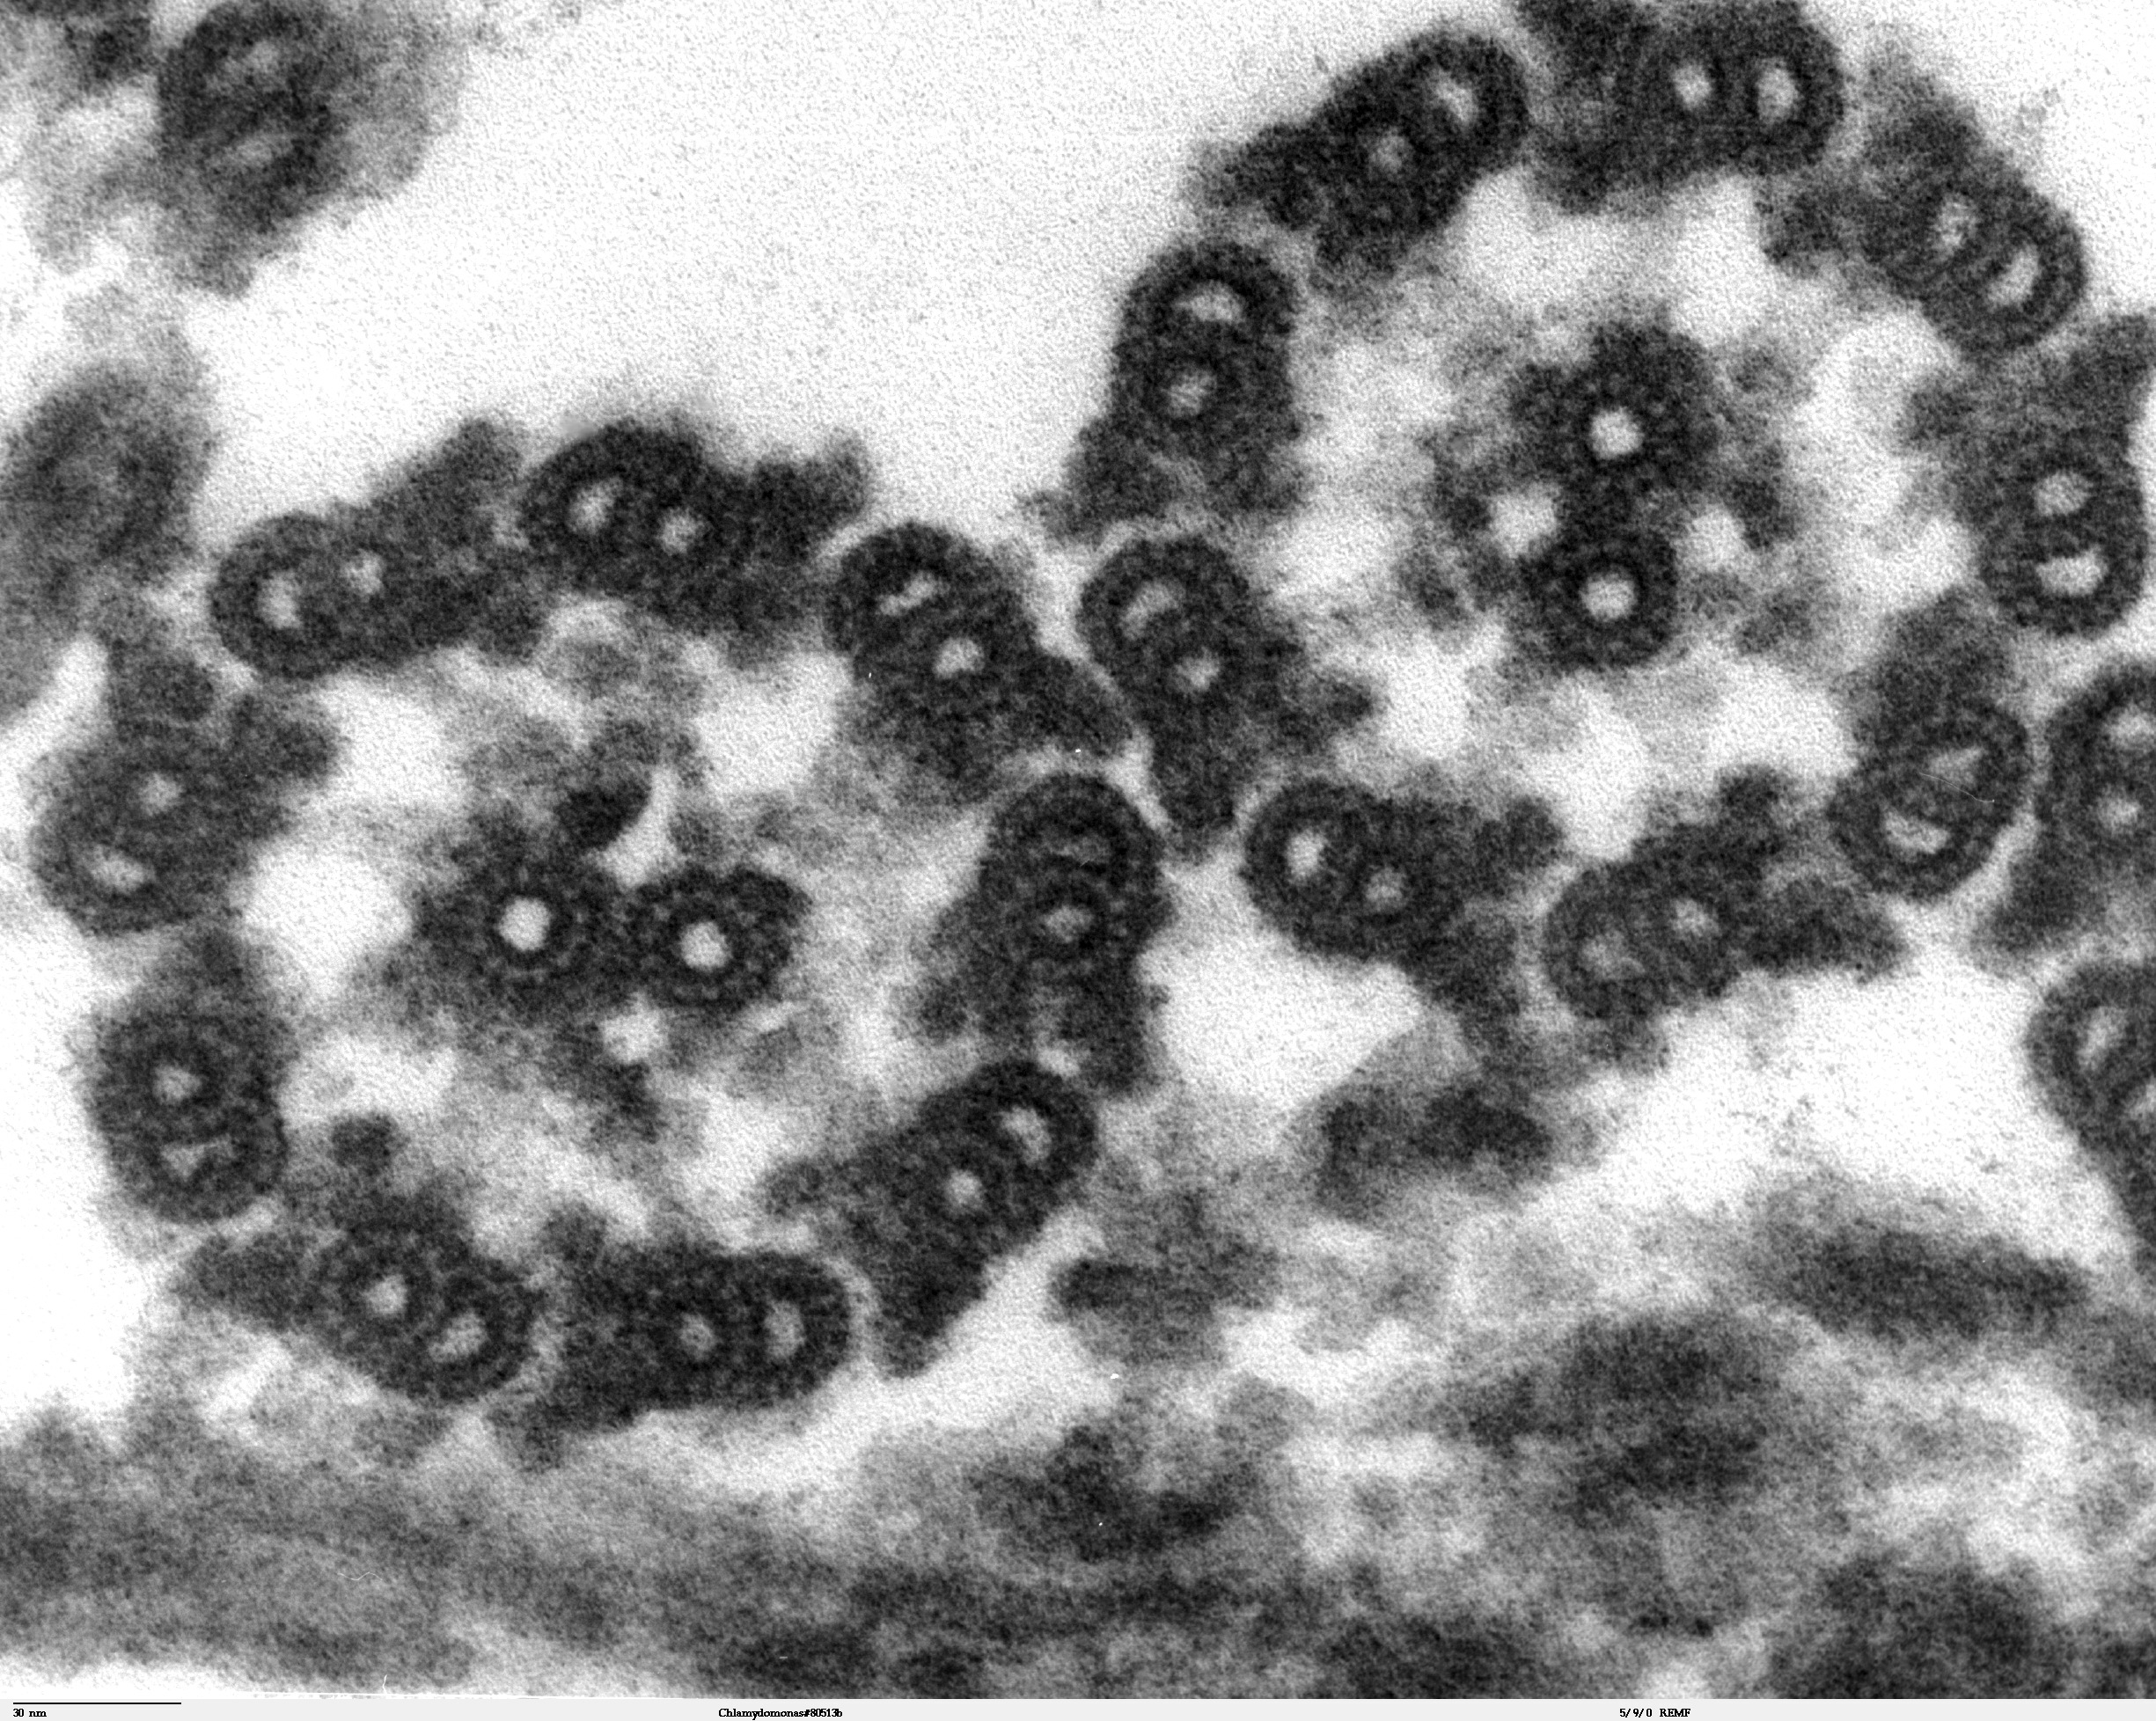
\includegraphics[width=\linewidth]{../../img/Chlamydomonas_TEM_17}

        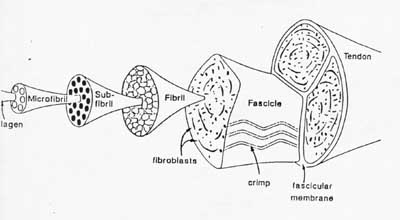
\includegraphics[width=\linewidth]{../../img/ligten2.jpg}

        \uncover<2->{
        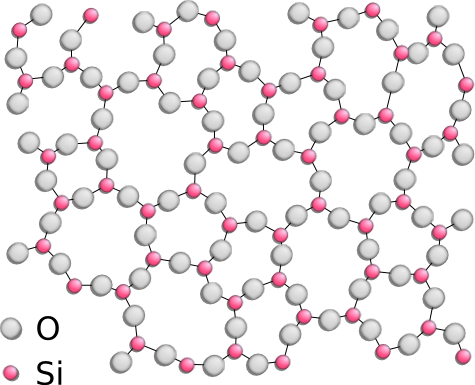
\includegraphics[width=\linewidth]{../../img/Silica}
        }

        \uncover<3->{
        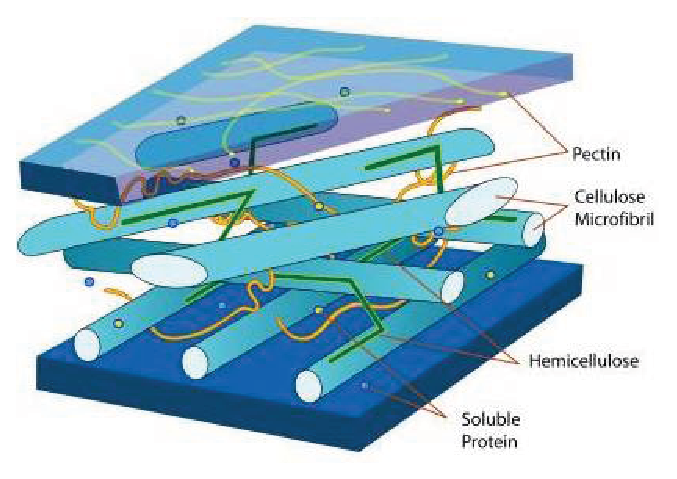
\includegraphics[width=\linewidth]{../../img/crosslink}
        }
    \end{column}
    \end{columns}
\end{frame}

\begin{frame}{Terminology}
% \footnotesize
    \begin{definition}[Over-constrained system]
        More constraint equations than primitive variables, modulo trivial motions of the ambient space. Generically, this means no realizations.
    \end{definition}
    % E.g., for 2D bar-joint, $|E|>2|V|-3$.

    \pause
    \begin{definition}[Independent system]
        No subsystem is over-constrained. Generically,  there exists some realization.
    \end{definition}

    \pause
    \begin{definition}[Rigid system]
        % Generically, there are finitely many realizations.
        There are finitely many realizations.
    \end{definition}

    \pause
    Can we efficiently find a realization?

    Doubly exponential in the size of the largest subsystem that must be solved simultaneously.

    % Questions:
    % \begin{itemize}
    % \footnotesize
    %     \item Can we classify a system as one of the above?
    %     % \item Given a constraint system, does there exist a realization? If the solution is real.
    %     % \item How many realizations? Finitely many if it's rigid.
    %     \item Can we find it efficiently?
    % \end{itemize}

    % The cost of solving is doubly exponential to the size of the largest subsystem that must be simultaneously solved.
\end{frame}

\begin{frame}{Combinatorics}
    Motivation: recursively decompose a system into independently solvable subsystems.

    \pause
    \n

    To do this we no longer care about the system, but rather the underlying combinatorics.

    \begin{definition}[Constraint graph]
        The underlying hypergraph of a geometric constraint system. Vertices represent the \term{geometric primitives} and hyperedges represent the \term{constraints}.
    \end{definition}

    \pause
    Combinatorial rigidity translates the properties of systems (over-constrained, independent, rigid) into properties of the underlying constraint graph, generically.
\end{frame}

\begin{frame}{Bar-Joint}
    Our results apply in the general setting, but for ease of exposition, we'll be restricting ourselves to bar-joint.

    \begin{definition}[Bar-joint system]
        Primitives: Points.
        Constraints: Distances.
    \end{definition}

    Distance is a binary relation on points, therefore the constraint graph is simply a graph.

    \begin{figure}
        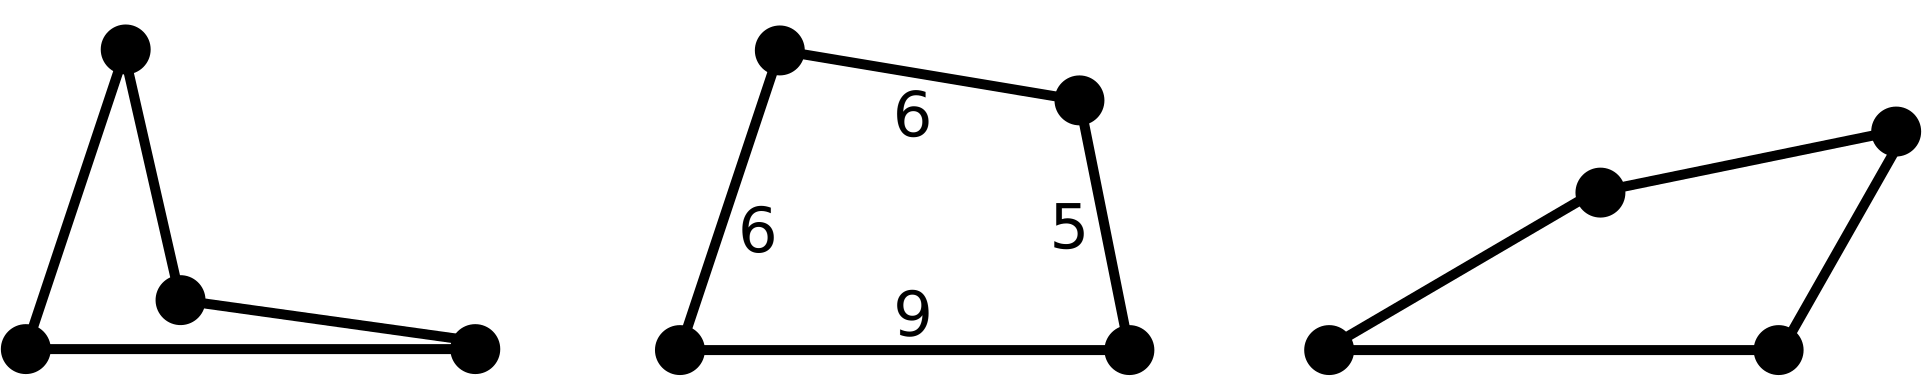
\includegraphics[width=\linewidth]{../../img/svg/barjoint_illustration_simple}
    \end{figure}
\end{frame}


\section{DR-Planning}
\begin{frame}{DR-Planning}
    \begin{definition}[Decomposition-recombination (DR-) plan]
        A \emph{DR-plan} of constraint graph $G$ is a forest where:
        \begin{itemize}
            \item Each node is a rigid subgraph of $G$.
            \item A root node is a maximal rigid subgraph.
            \item An internal node is the union of its children.
            \item A leaf node is a single constraint and the involved primitives.
        \end{itemize}
    \end{definition}

    % \todo{Probably irrelevant, examples, two for the same graph}
    % This is purely combinatorial, dealing with the underlying graph. The actual constraint don't change the output.
\end{frame}

\begin{frame}{Example DR-Plans: $C_2\times C_3$}
    \begin{figure}
        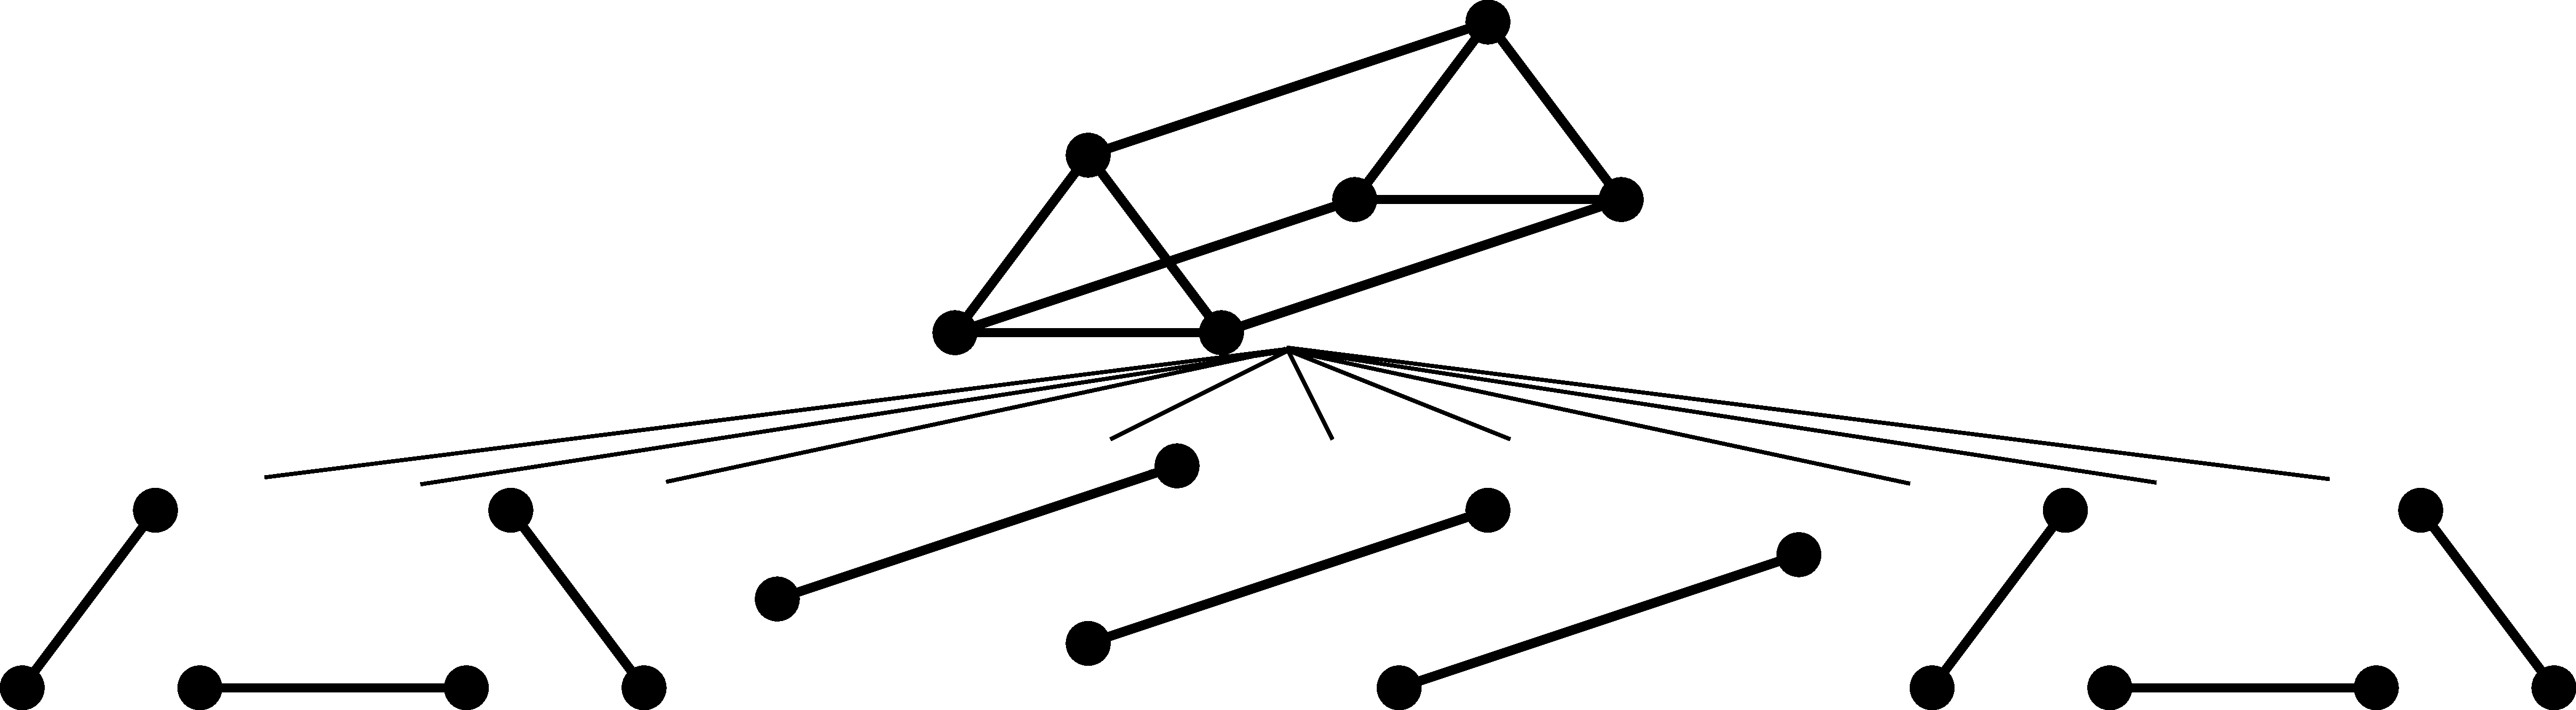
\includegraphics[width=0.9\linewidth]{../../img/svg/drplanning_illustration_a}

        \pause
        \n

        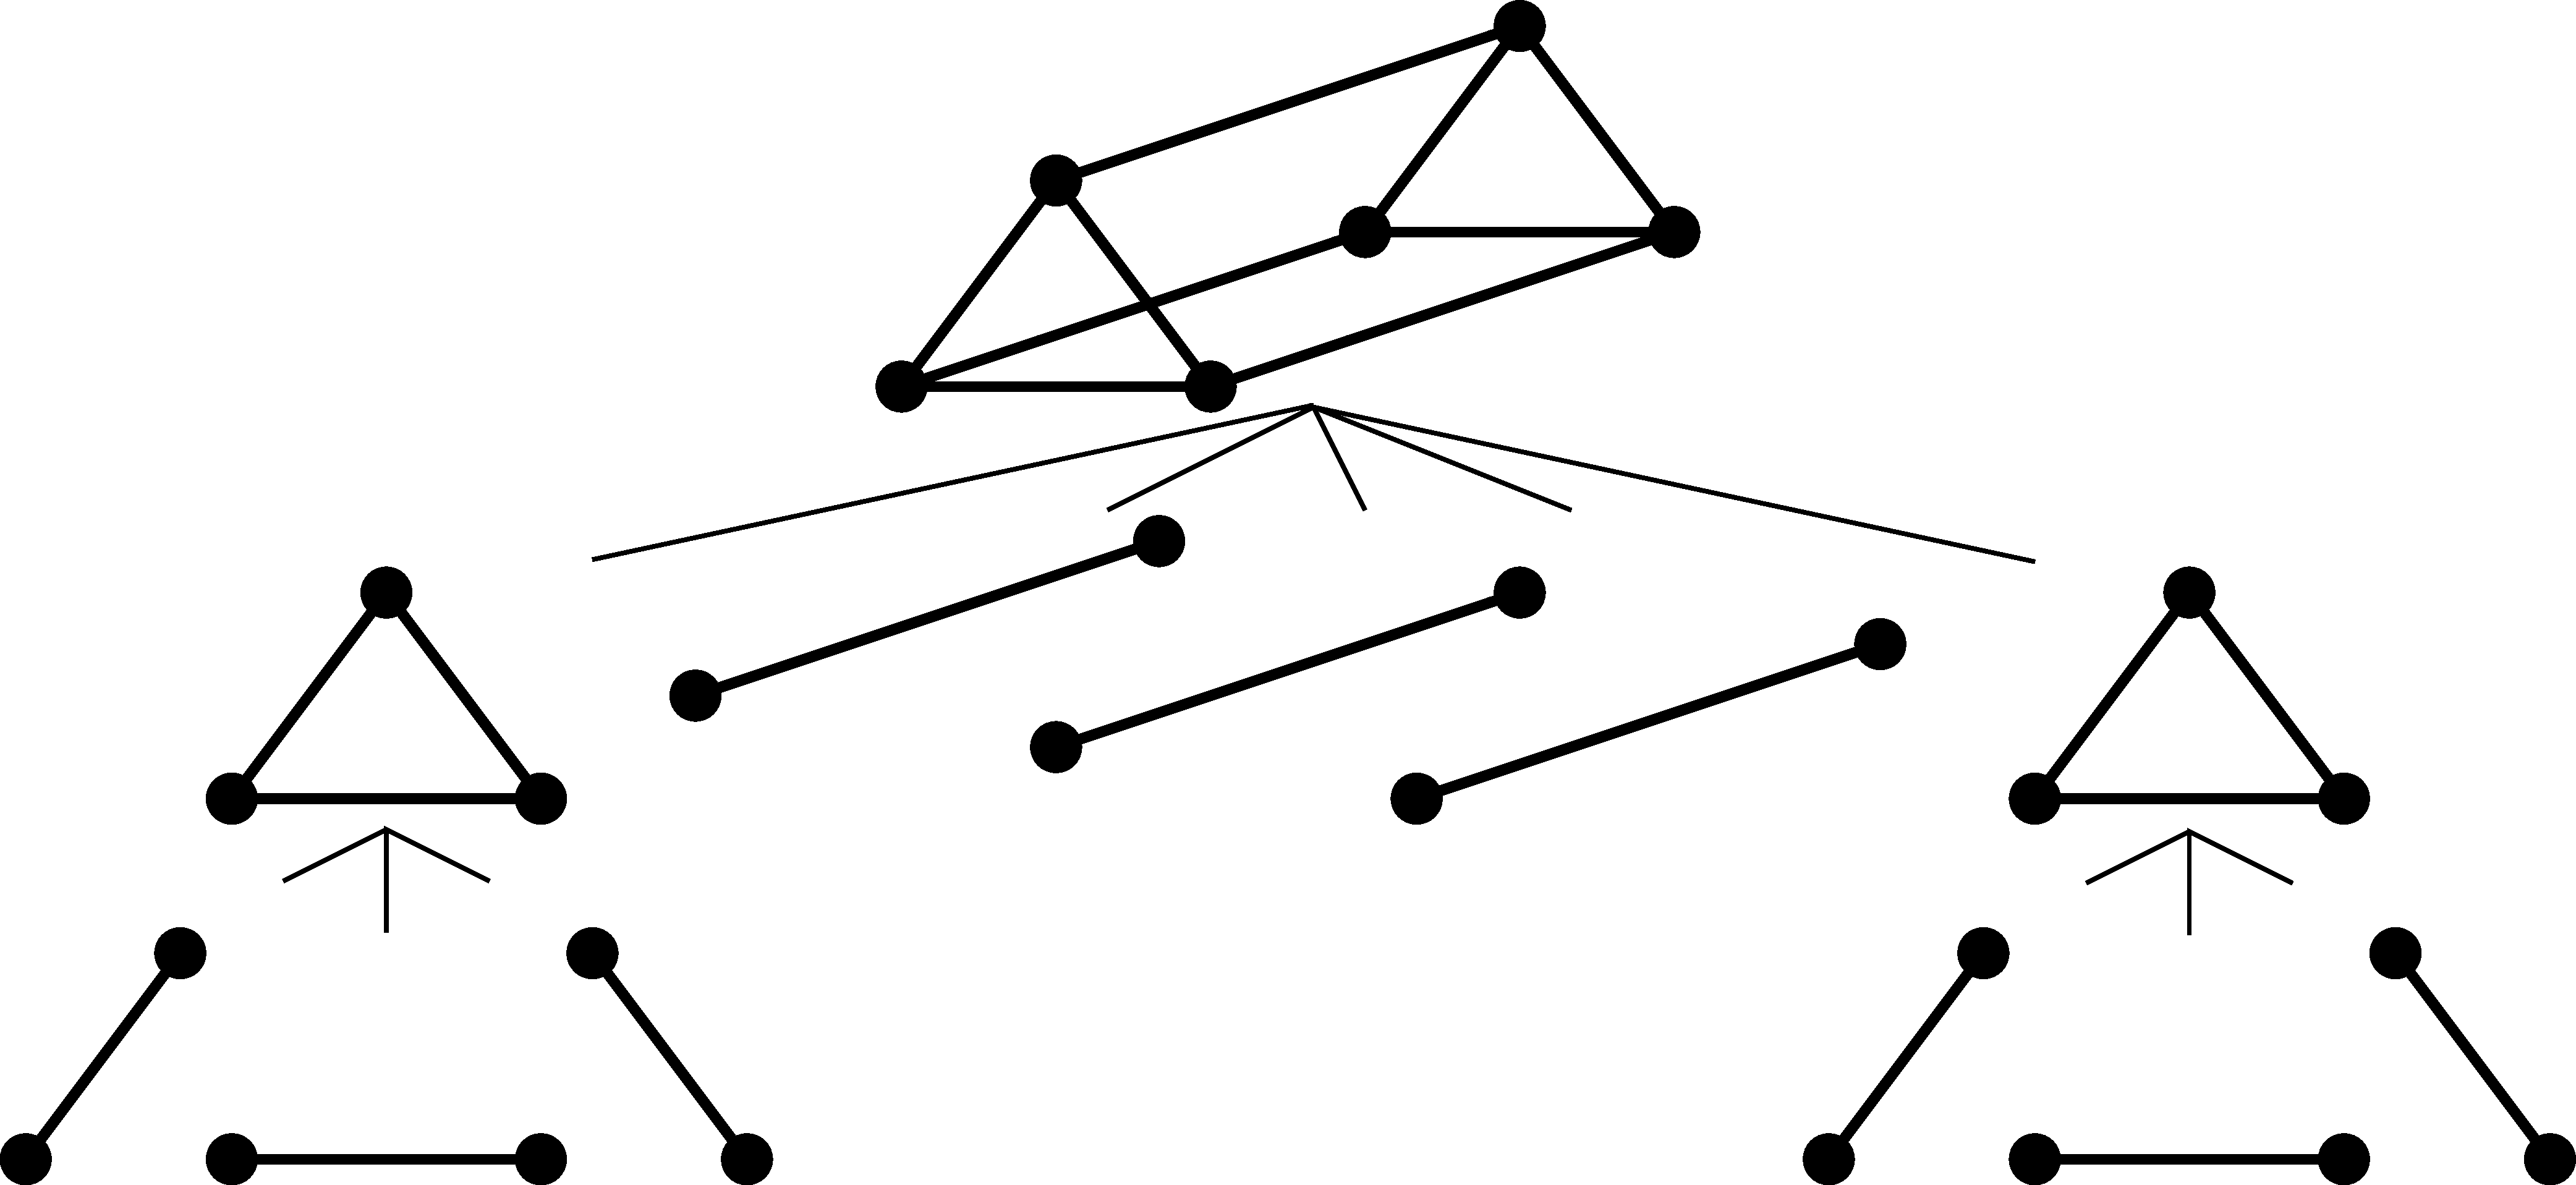
\includegraphics[width=0.9\linewidth]{../../img/svg/drplanning_illustration_b}
    \end{figure}
\end{frame}

\begin{frame}{Optimal DR-Plan}
    An \emph{optimal DR-plan} minimizes the maximum fan-in.
    % Corresponds to the largest subsystem that needs to be solved simultaneously.

    \pause
    \n

    In general, finding optimal is NP-hard.

    % If the graph is not independent, finding an optimal DR-plan is NP-hard in most cases, \emph{even} if rigidity is captured by an underlying sparsity condition (as in 2D bar-joint.)
    % \cite{lomonosov2004thesis}
    % % \footfullcite{lomonosov2004graph}

    \begin{figure}\centering
        \begin{subfigure}{.35\linewidth}\centering
            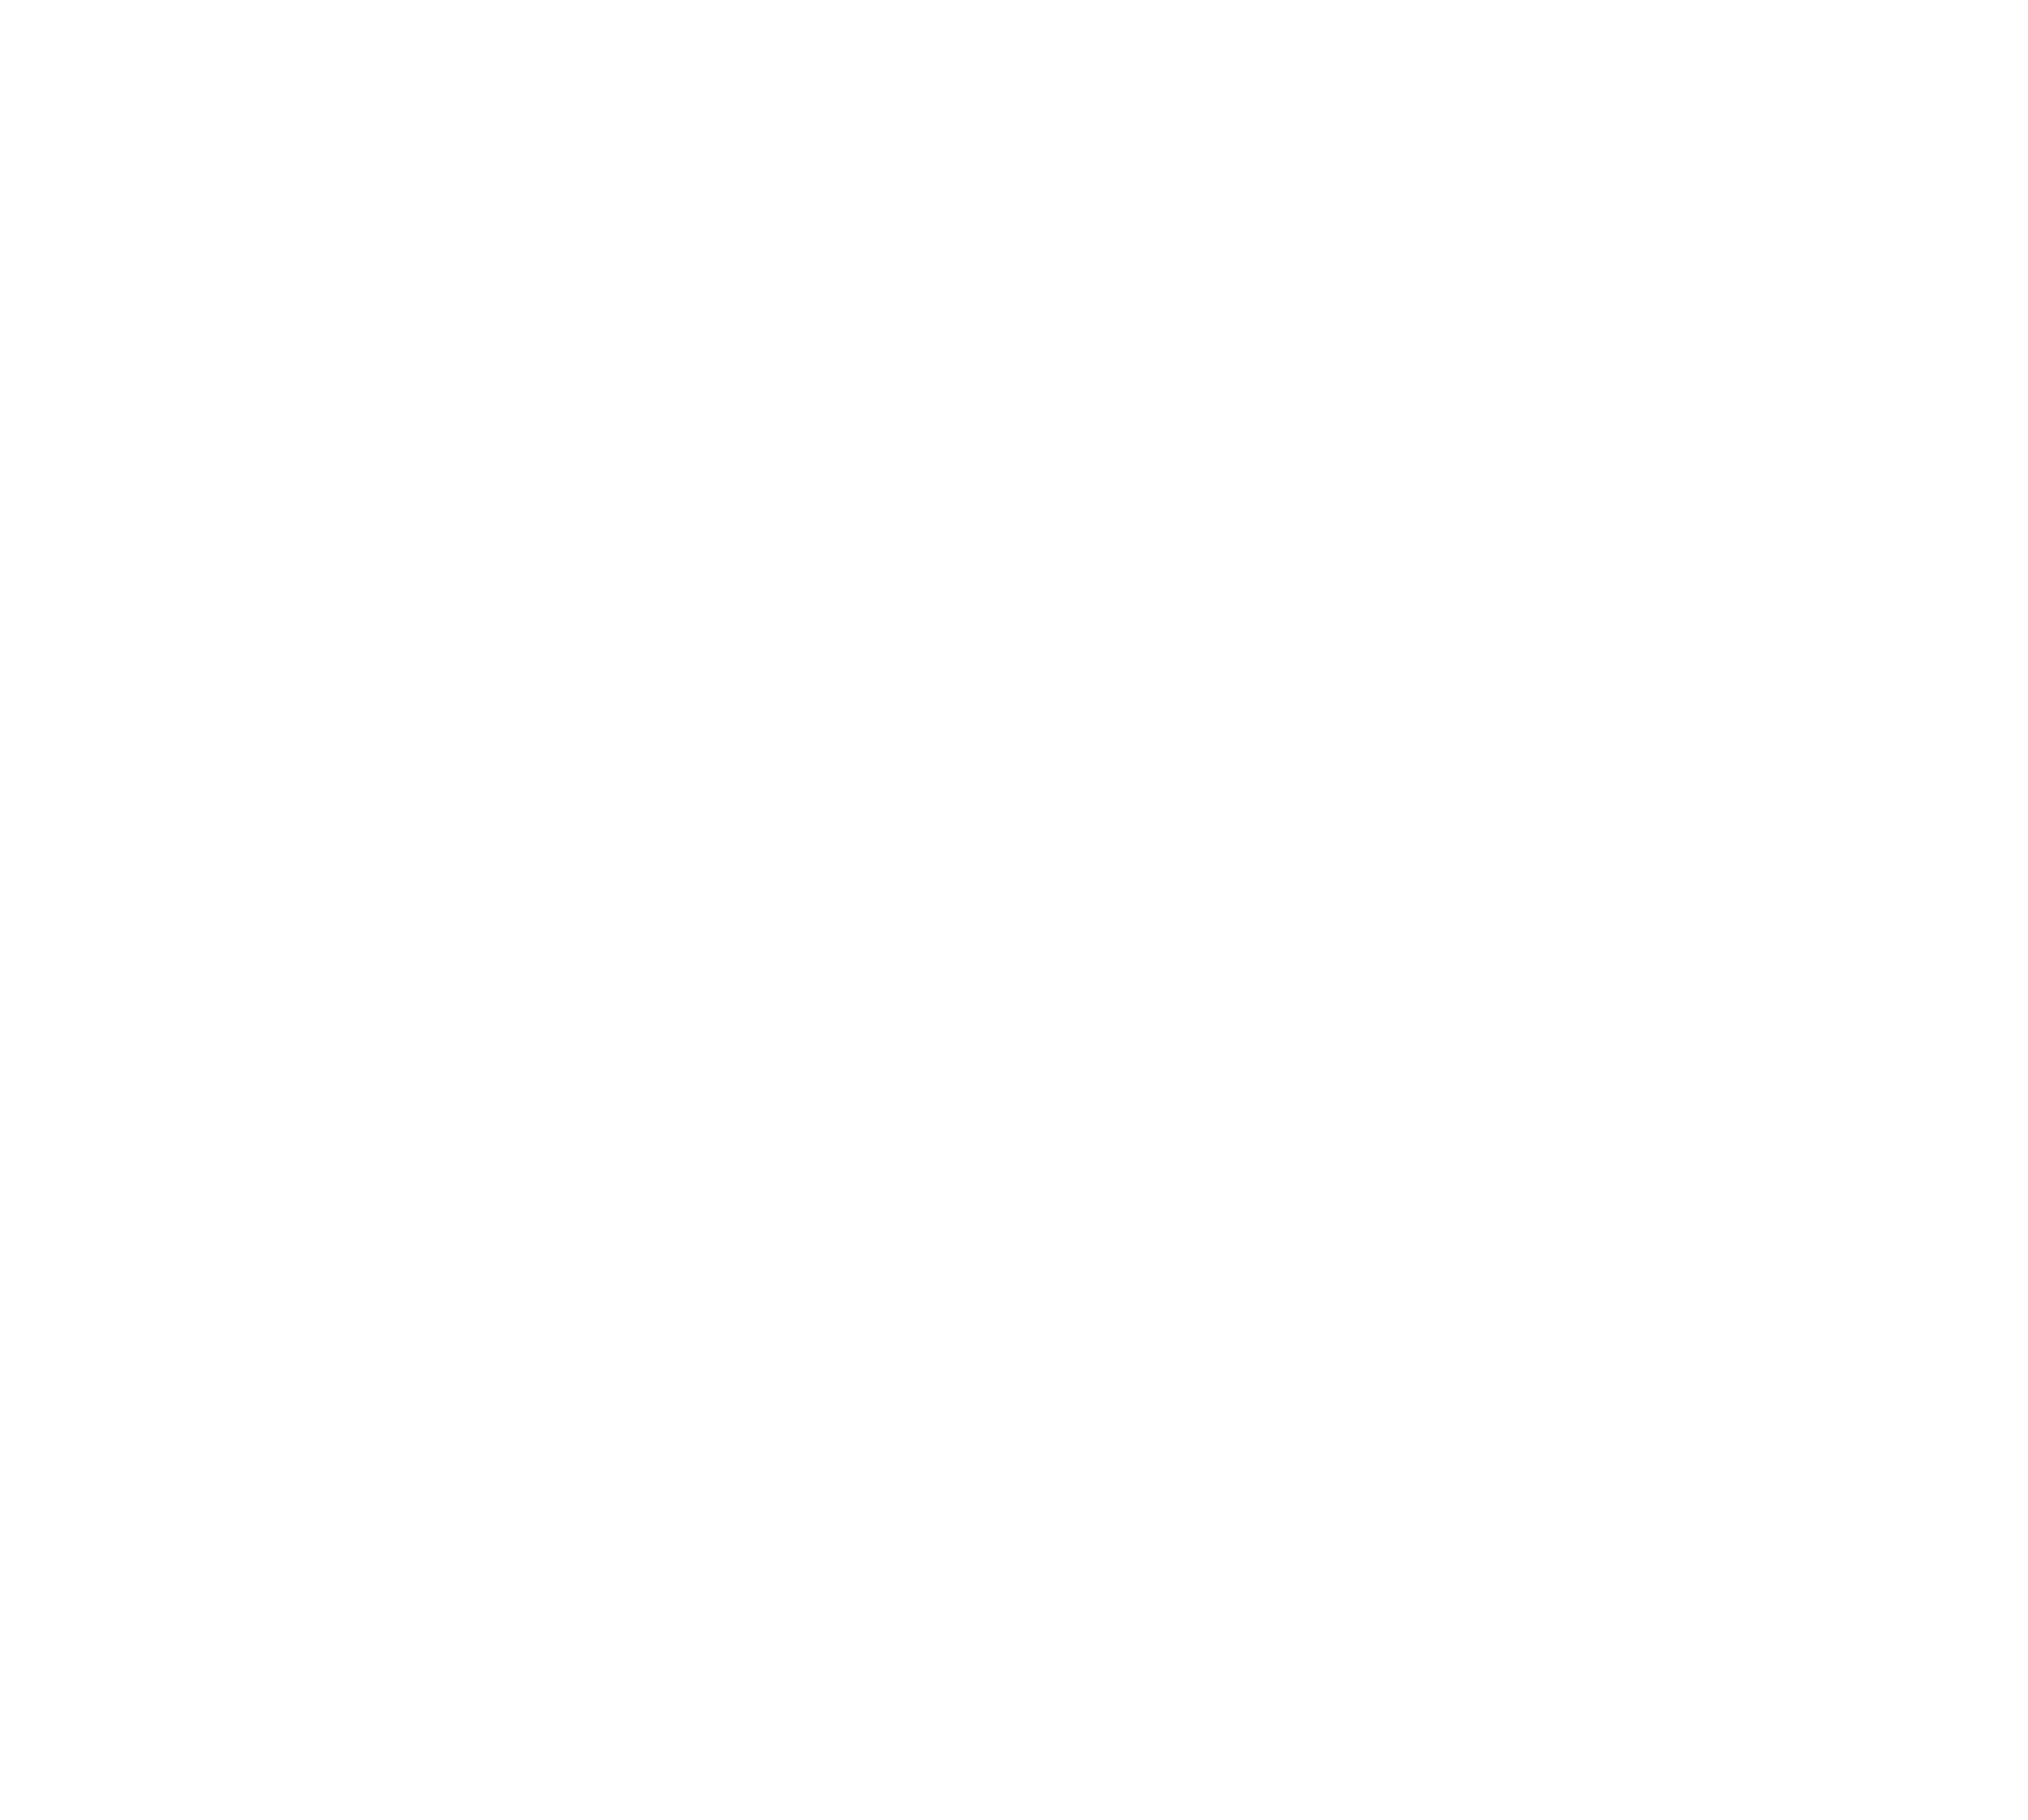
\includegraphics[width=\linewidth]{../../img/svg/new_overconstrained_optimal}
        \end{subfigure}
        %
        \hspace{.1\linewidth}
        \begin{subfigure}{.35\linewidth}\centering
            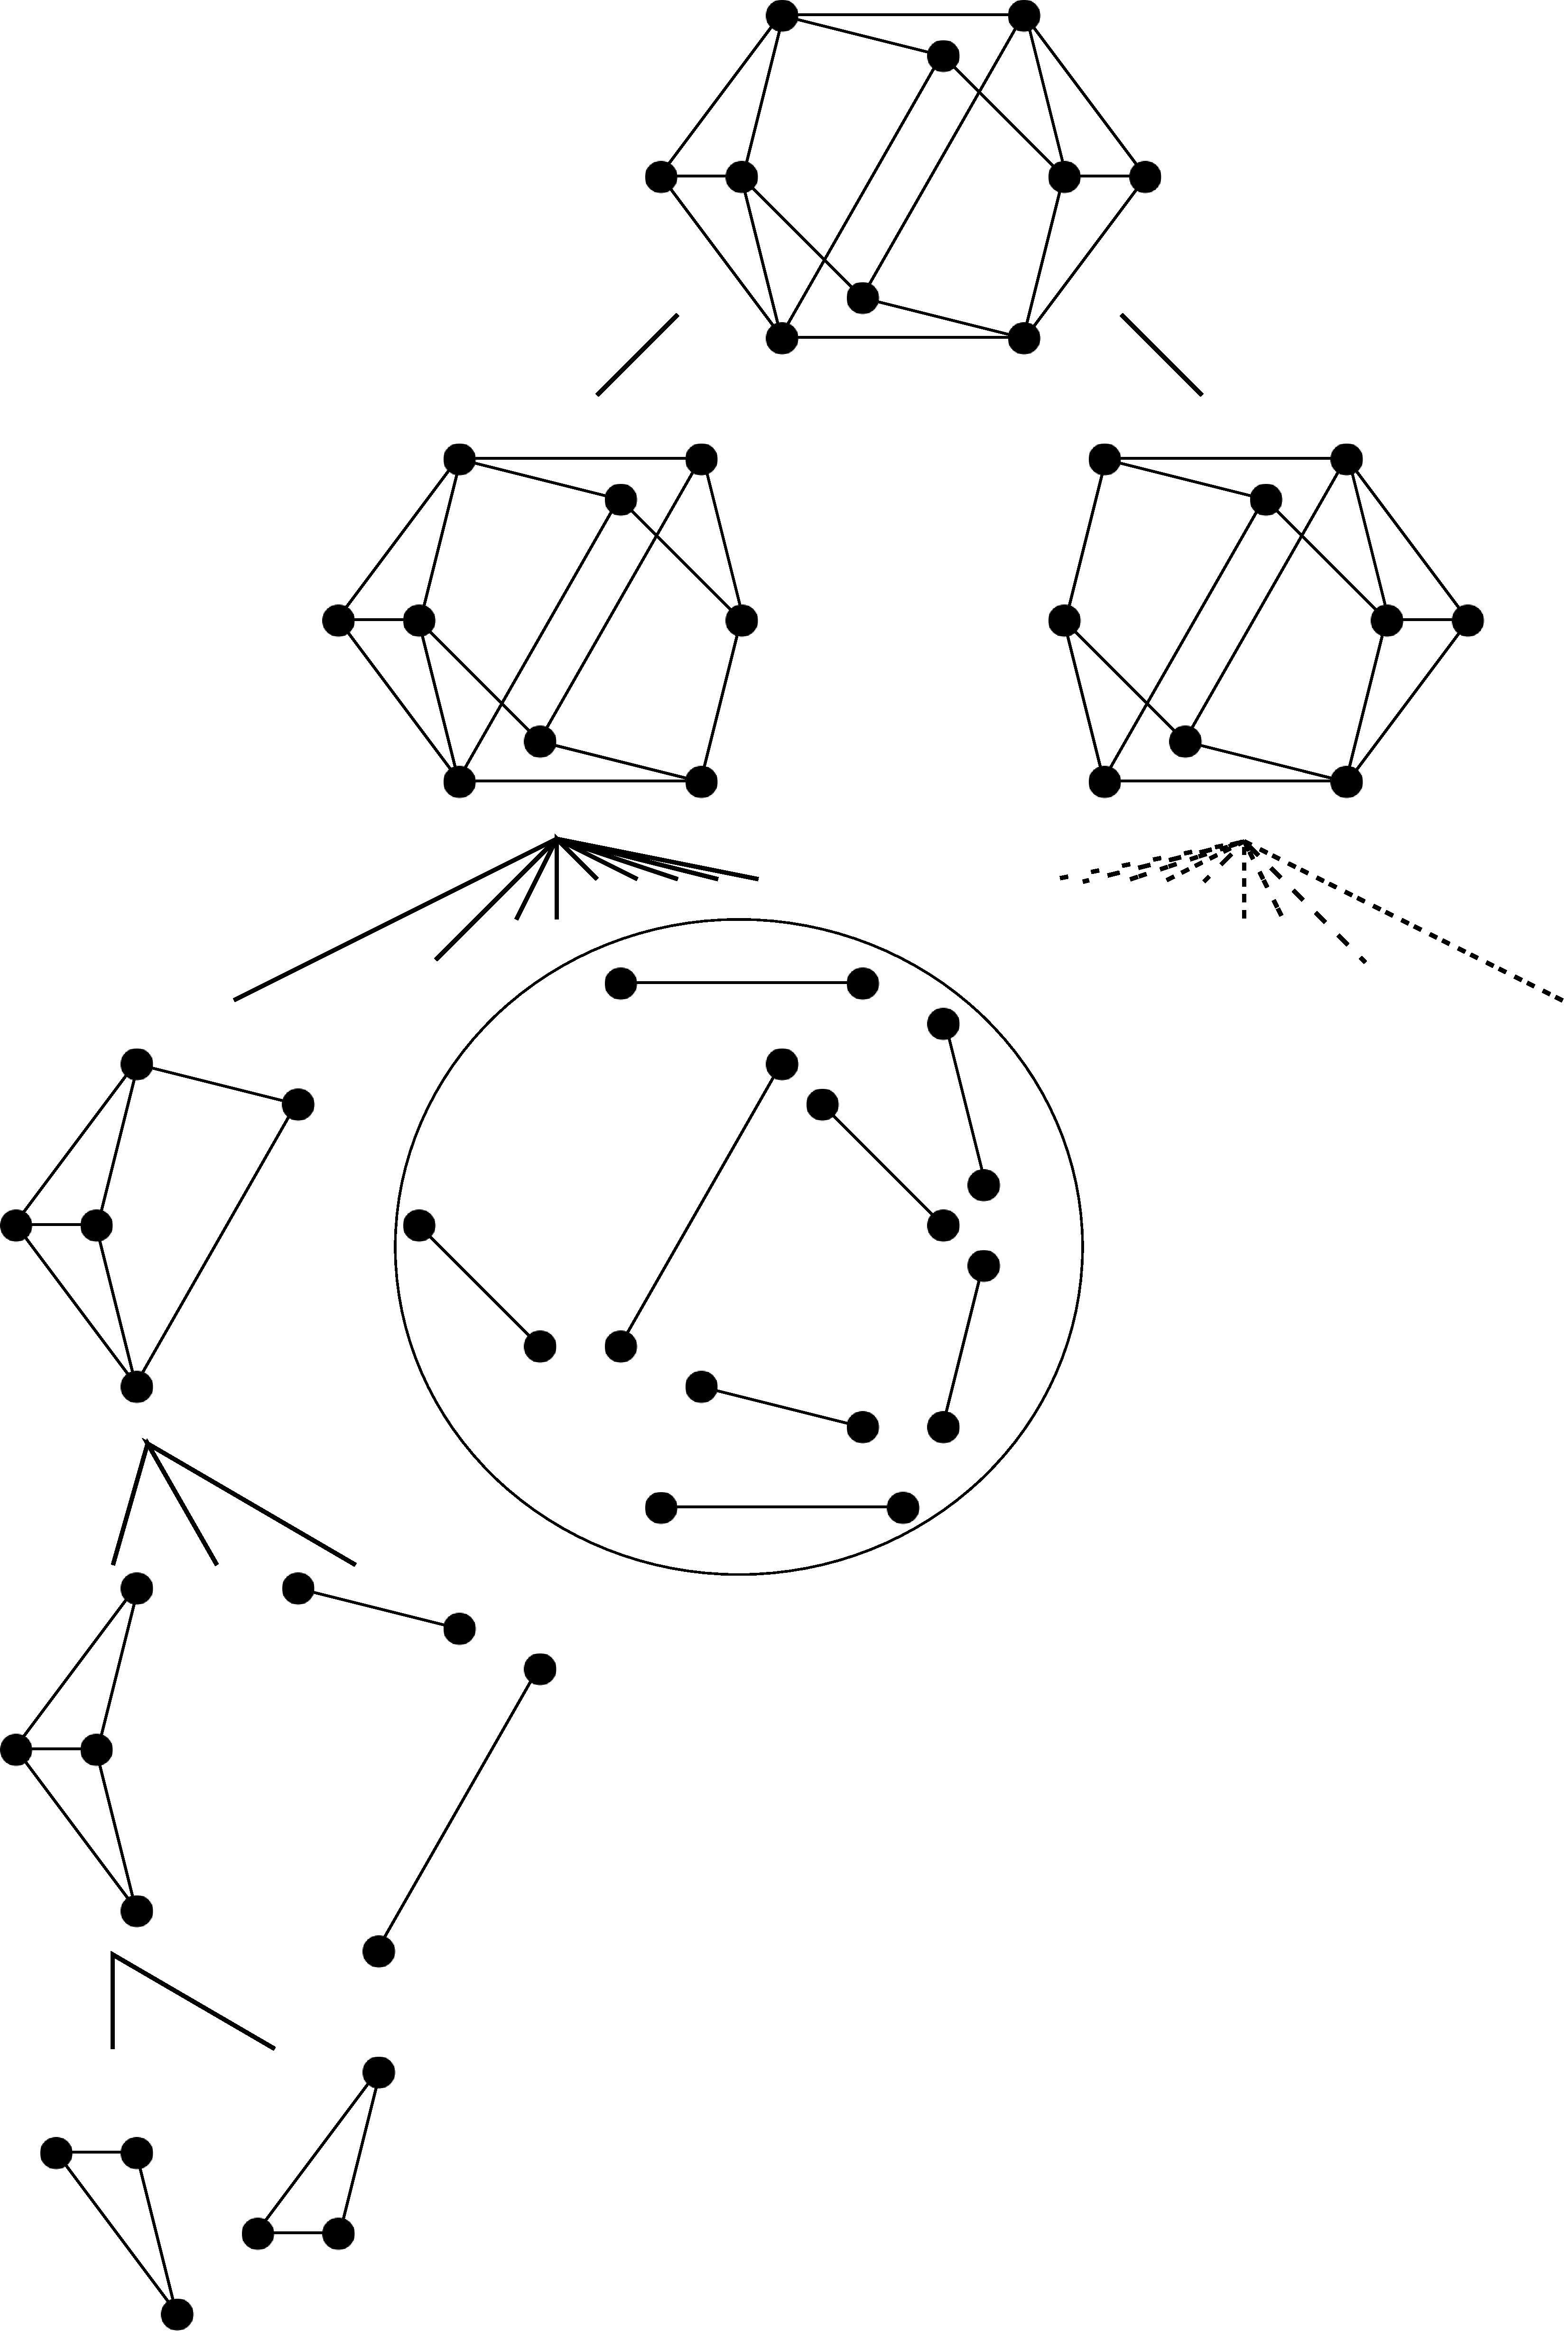
\includegraphics[width=\linewidth]{../../img/svg/new_overconstrained_not_optimal}
        \end{subfigure}
    \end{figure}
    % \begin{figure}\centering
    %     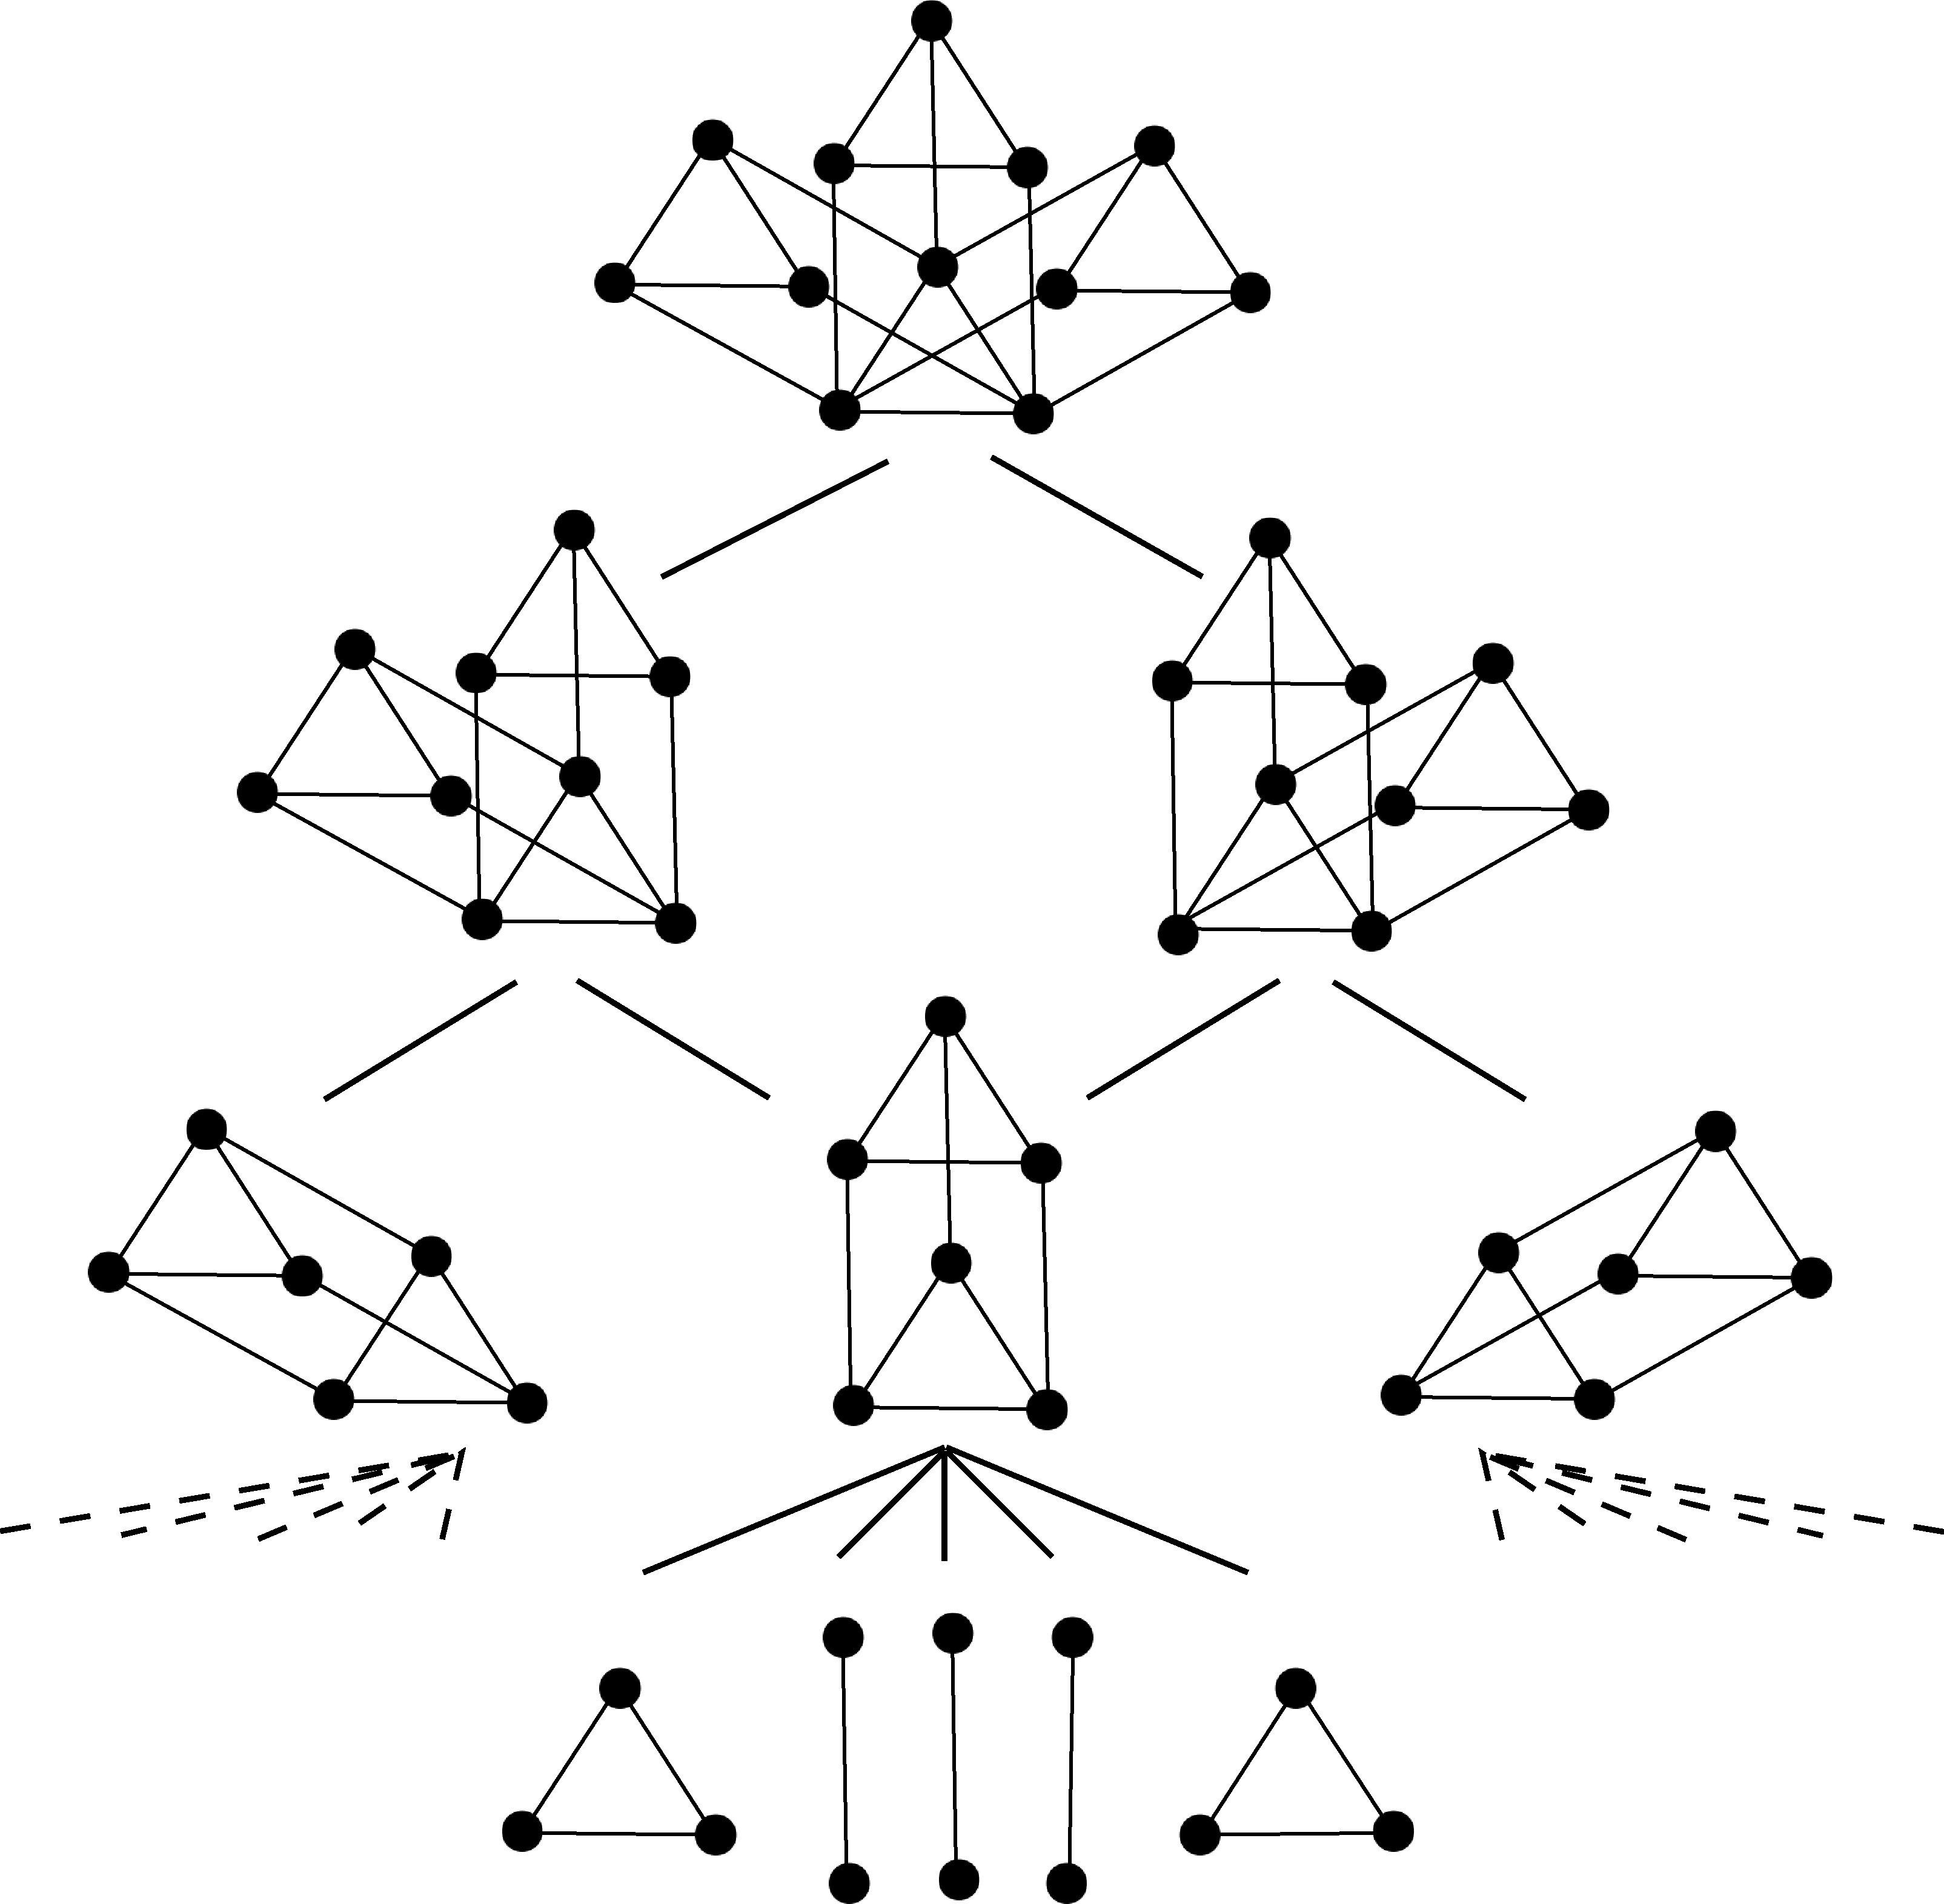
\includegraphics[width=.5\linewidth]{../../img/svg/3xc2c3_candrp_full}
    % \end{figure}
\end{frame}

\begin{frame}{Uses of DR-Planning}
    \begin{itemize}
    \setlength\itemsep{1em}
        \item Determining complexity of solving.
        \item Decomposition of the stress and flex matrices.
        \item Under-constrained completion.
        \item Interactive removal of over-constraints.
    \end{itemize}

    % Determining complexity of solving.

    % \n

    % Under-constrained completion.

    % \n

    % Interactive removal of over-constraints.

    % \n

    % Decomposition of the stress and flex matrices.

    % ------------

    % \begin{itemize}
    %     \item Size of max fan-in is the size of the largest subsystem that has to be simultaneously solved, thus determining the complexity of solving.
    %     \item Figuring out how to complete under-constrained systems.
    %     \item Offering choices to remove over-constraints to get well-constrained.
    %     \item For those of you familiar, corresponds to a decomposition of the underlying rigidity matrix as well, giving decompositions of the flexes and self-stresses.
    % \end{itemize}
\end{frame}

\begin{frame}{History}
    2001: Formalized by Hoffman, Lomonosov, and Sitharam.~\cite{hoffman2001decompositionI}

    \n

    Late 1980's: Began with triangle-decomposable graphs. Corresponds to systems that can be triangularized and therefore have quadratic radical solutions (QRS).

    \n

    1990's-2000's: Older algorithms were \emph{bottom-up} and were based on maximum matching. E.g., Frontier. Made plans with some property other than optimality.

    \n

    2015: Our paper~\cite{baker2015optimal} contains a top-down $O(|V|^3)$ algorithm with a formal guarantee to find an optimal DR-plan, given some conditions.
\end{frame}



\section{Main Result: Optimal DR-Plan}
\begin{frame}{Summary of Results}
    If the system we're considering\ldots
    \begin{itemize}[<+->]
        \item Has an underlying abstract rigidity matroid $\to$ We can push the conceptual structures through.
        \item Is independent $\to$ We achieve optimality.
        \item Has an underlying sparsity matroid $\to$ We get a polynomial time algorithm.
    \end{itemize}

    \n

    \uncover<3->{
    For 2D bar-joint we have $O(|V|^3)$ time algorithm.
    }
\end{frame}

\begin{frame}{Canonical DR-Plan}
    % We introduce a canonical DR-plan, which is guaranteed to exist and to be optimal for independent graphs.

    \begin{columns}
    \begin{column}{0.495\textwidth}
        \begin{definition}[Canonical DR-plan]
            A DR-plan that satisfies the additional two properties:
            \begin{enumerate}
                \item Children are rigid vertex-maximal proper subgraphs (\rvmps) of the parent.
                \item If all pairs of \rvmps\ intersect trivially then all of them are children, otherwise exactly two that intersect non-trivially are children.
            \end{enumerate}
        \end{definition}

    \end{column}
    \begin{column}{0.475\textwidth}
        \begin{figure}\centering
            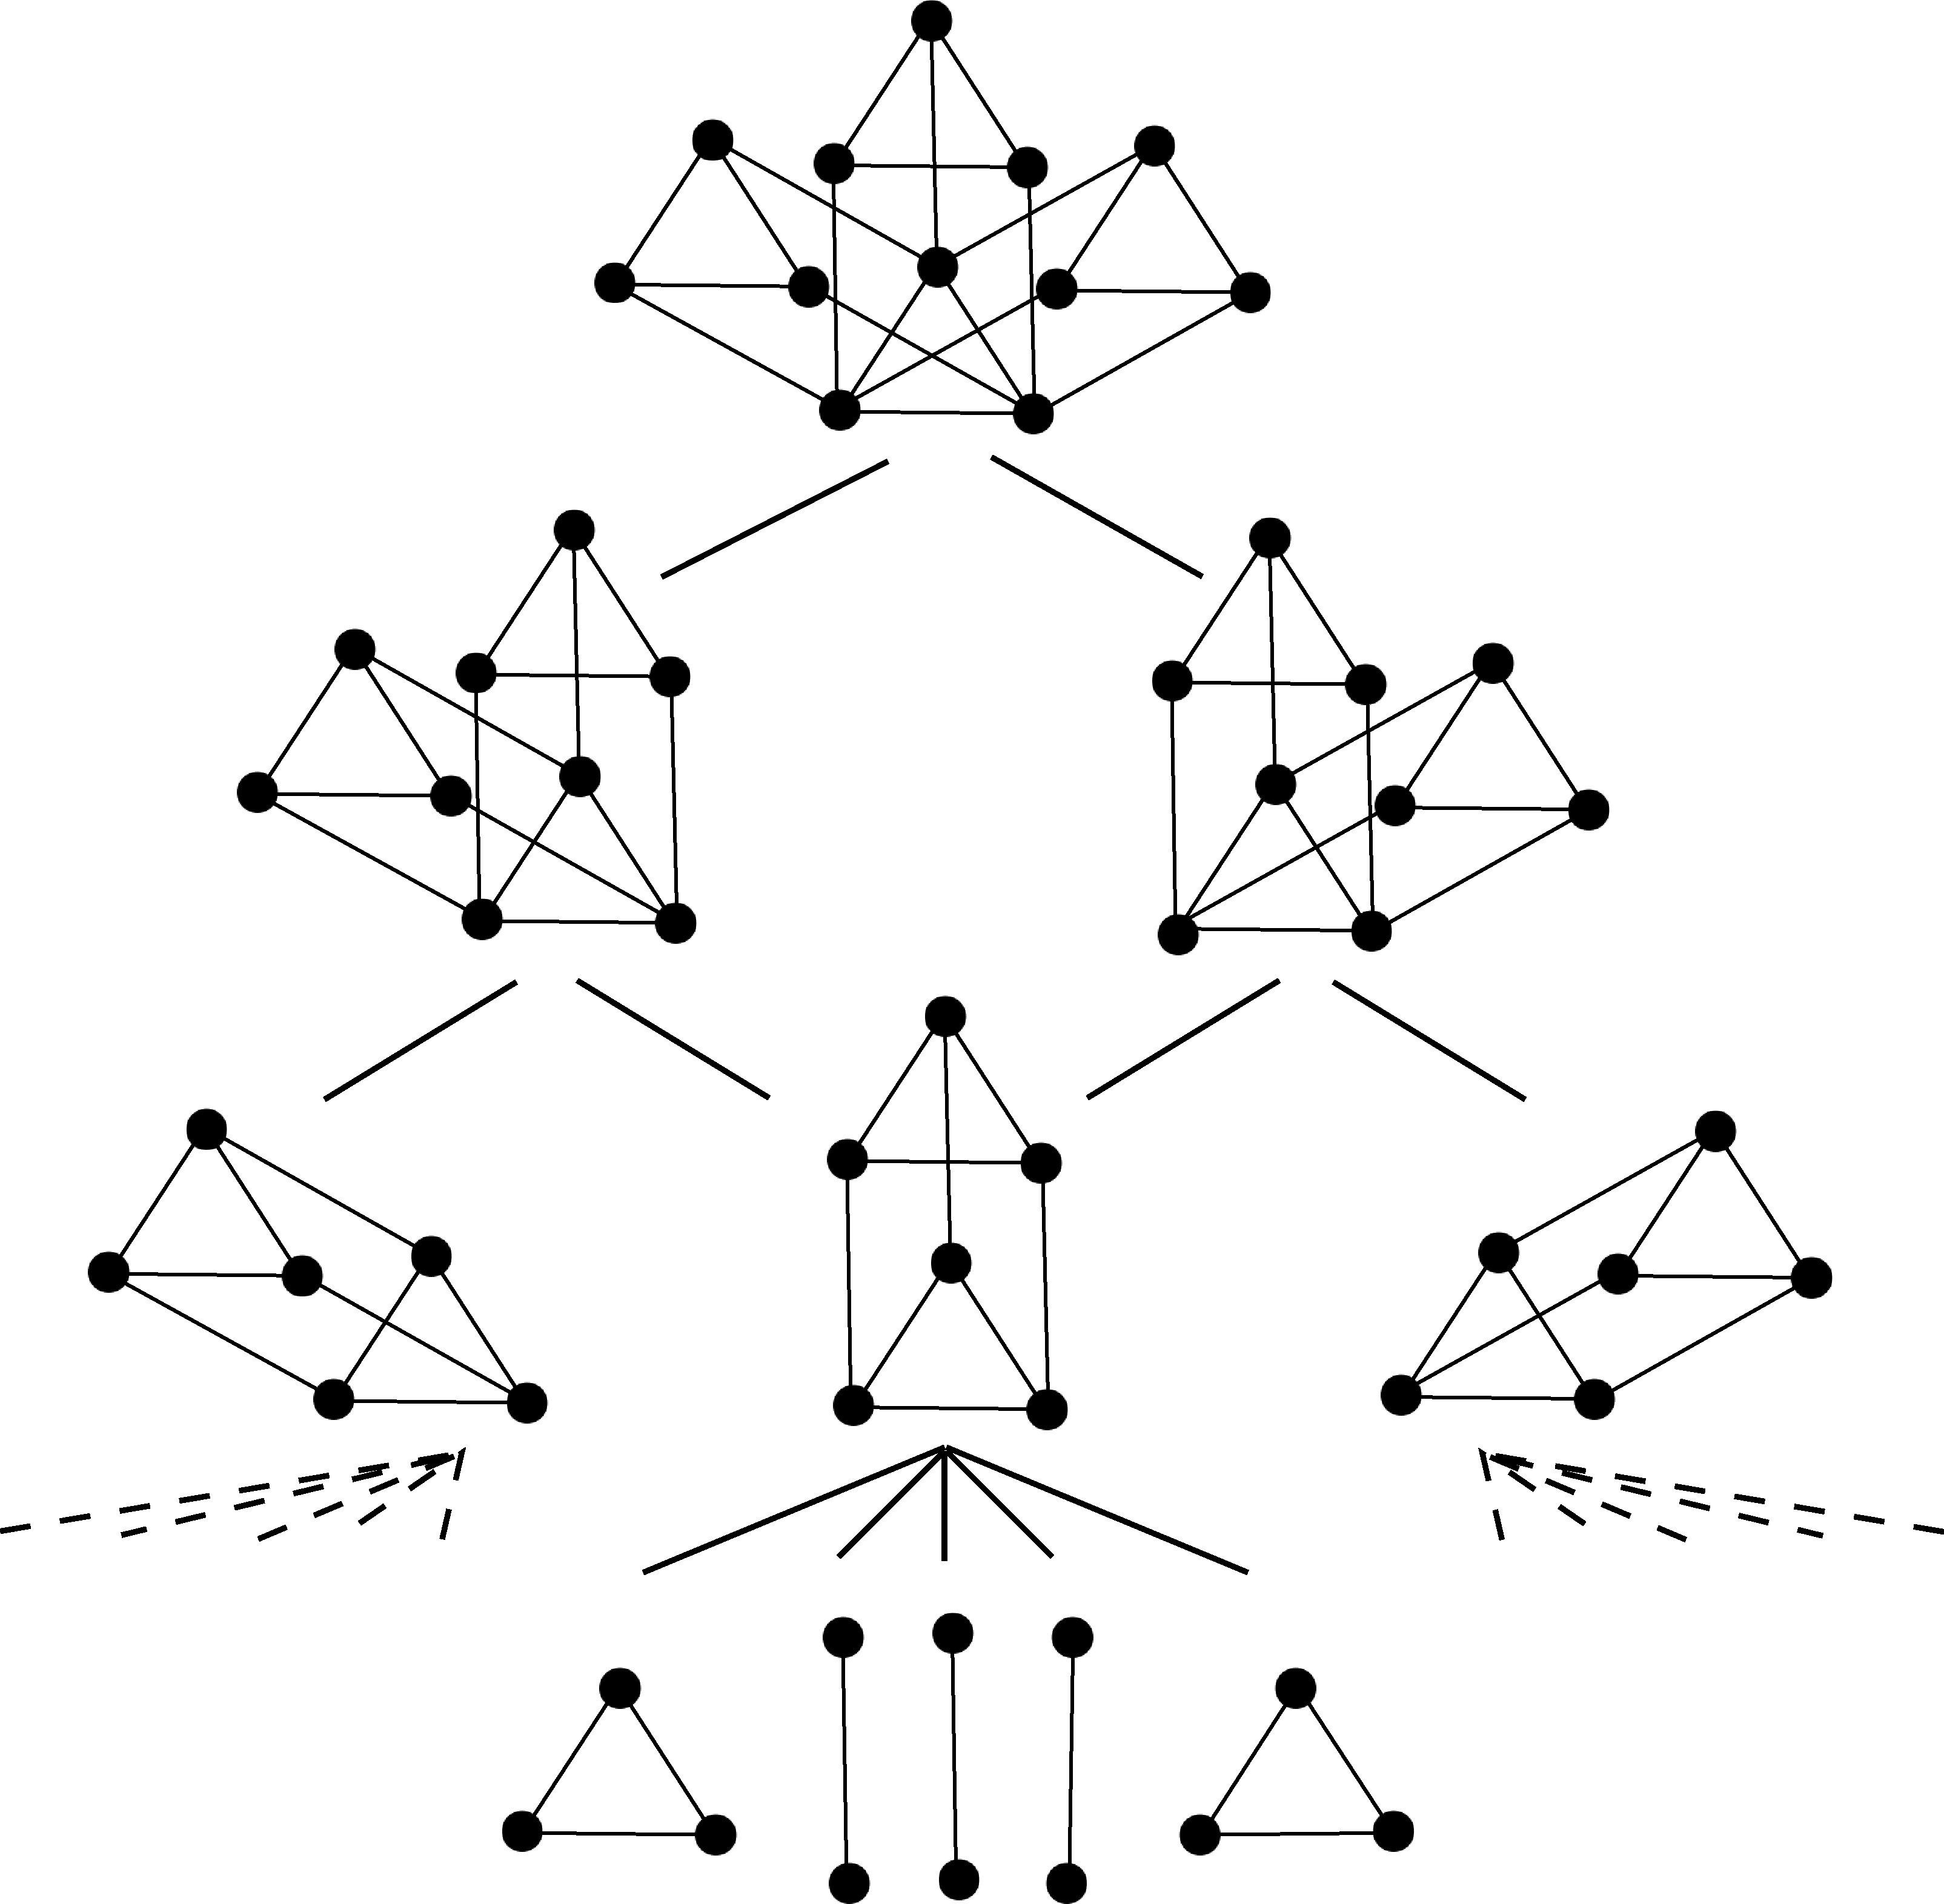
\includegraphics[width=\linewidth]{../../img/svg/3xc2c3_candrp_full}
            % 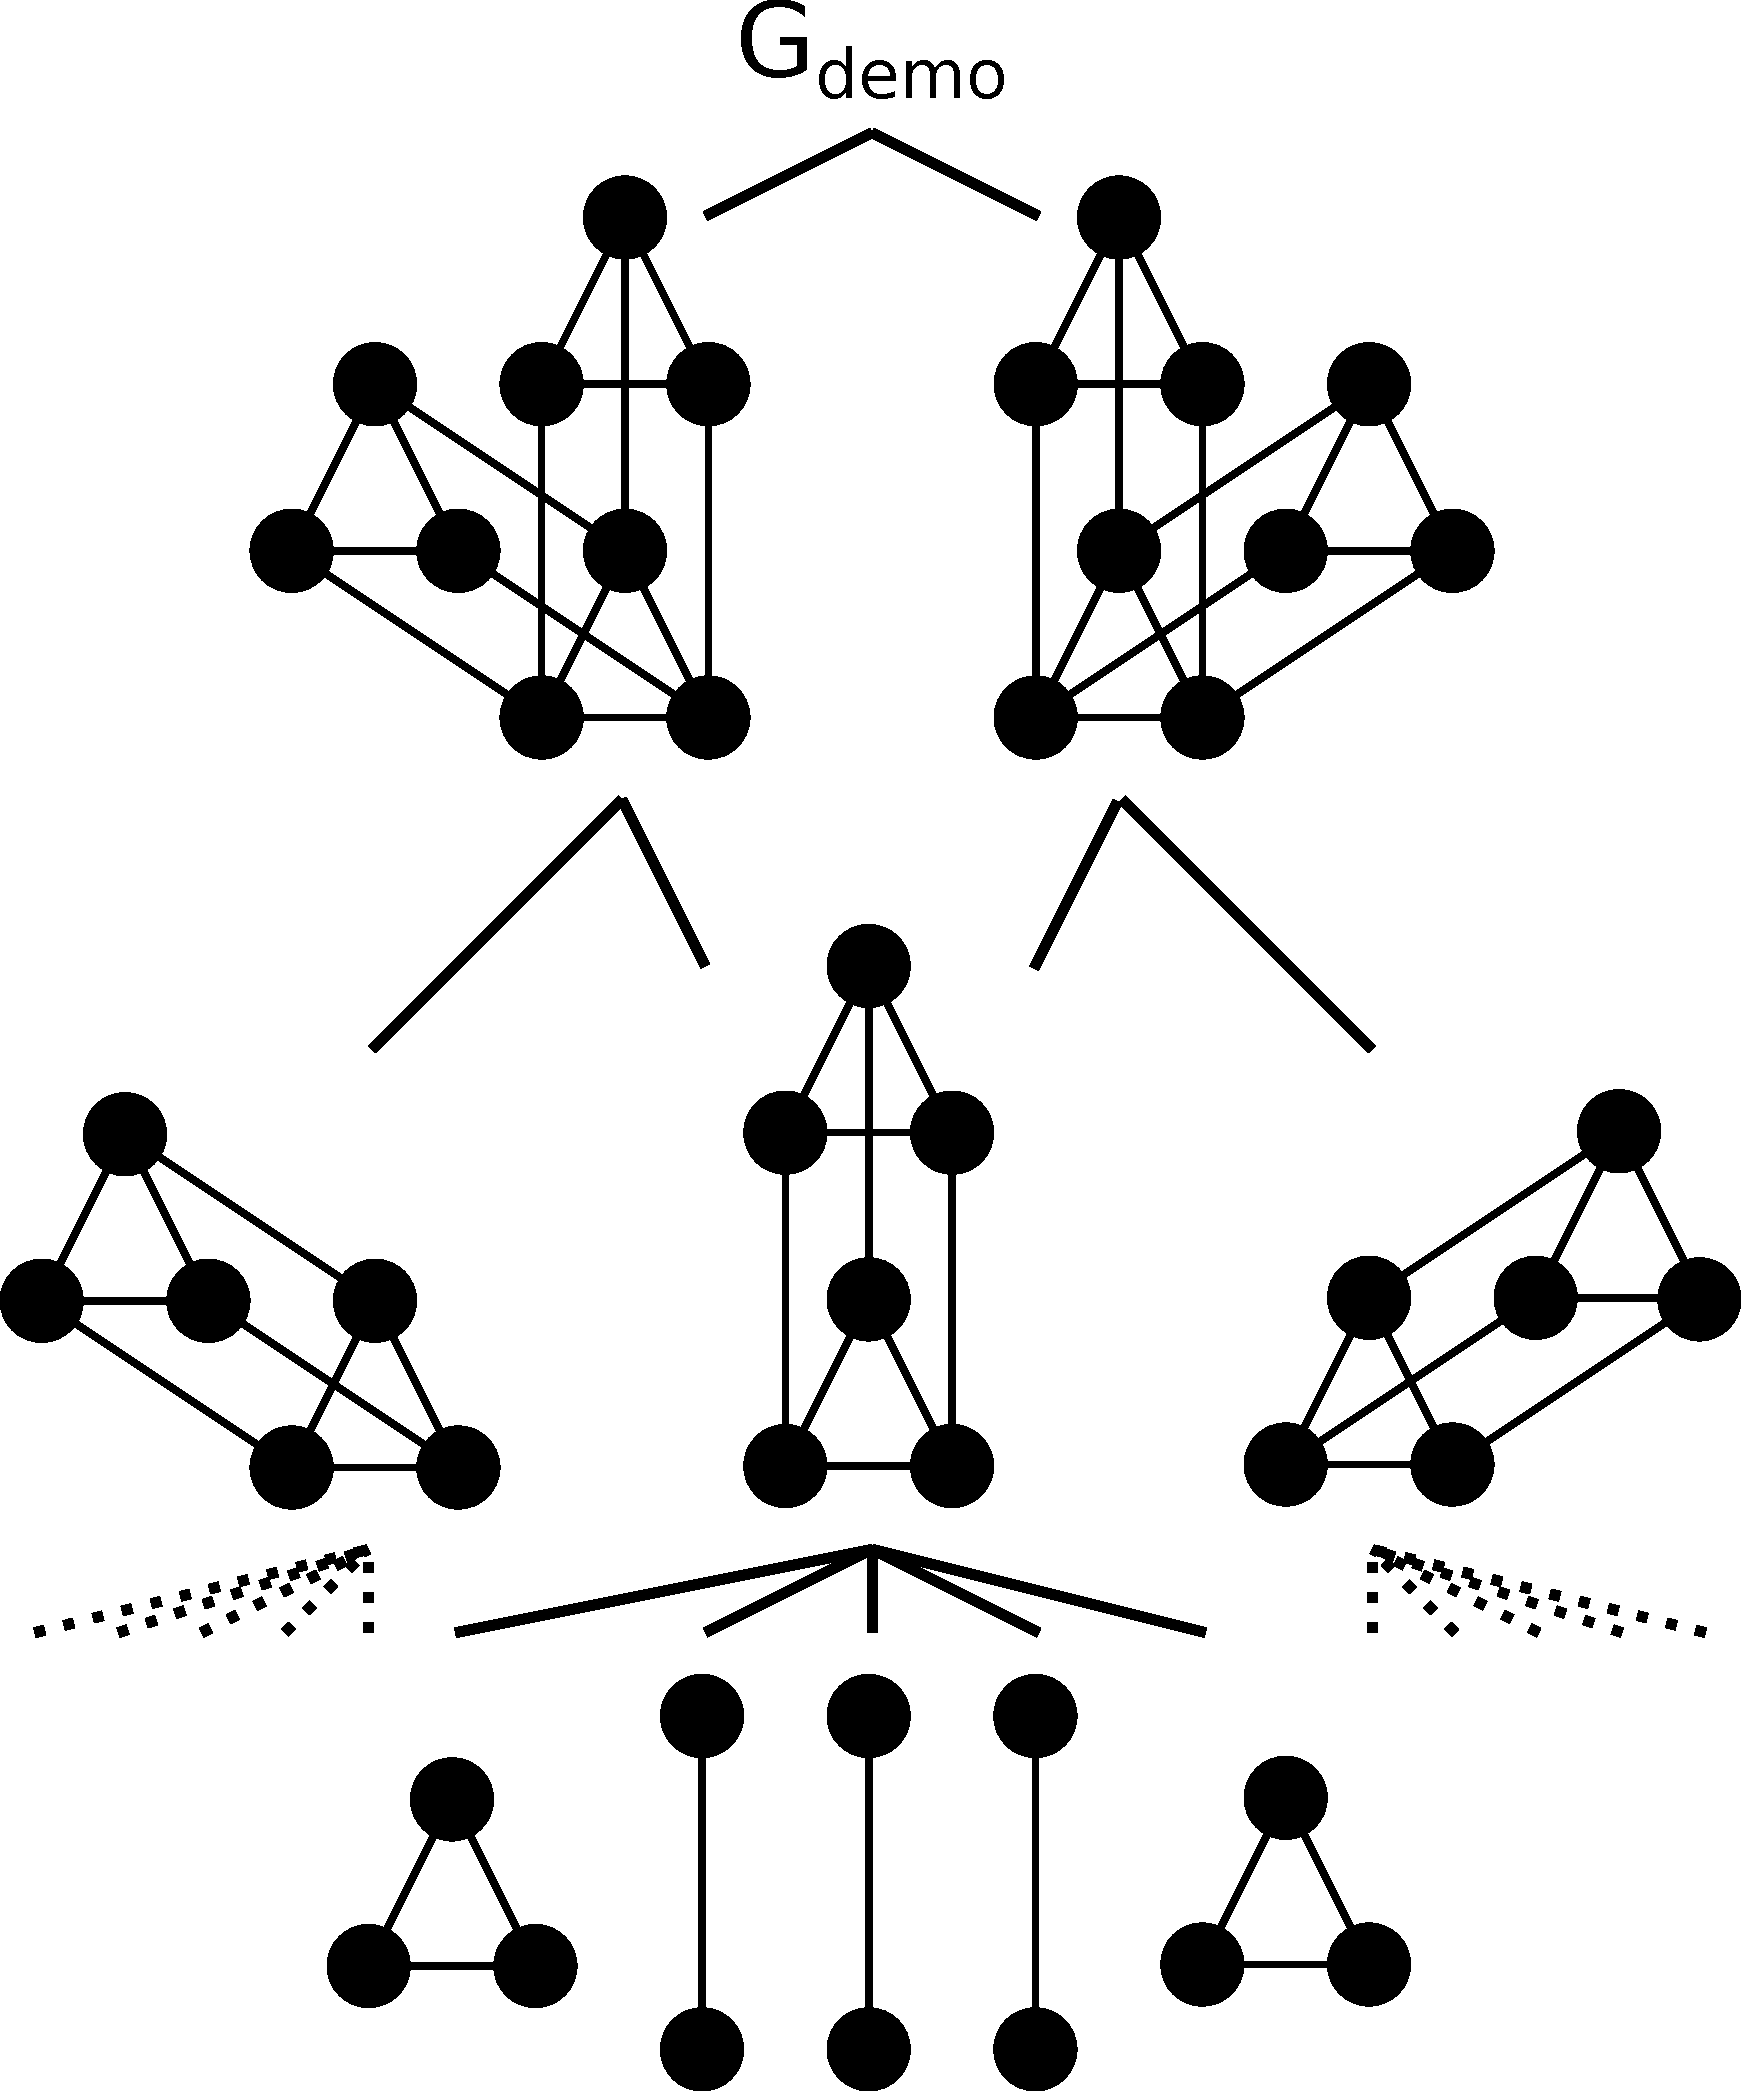
\includegraphics[width=\linewidth]{../../img/svg/3xc2c3_new_candrp}
        \end{figure}

    \end{column}
    \end{columns}

\end{frame}

\begin{frame}{Importance of Canonical DR-Plan}
    We restrict the space of DR-plans for the input to this special class of canonical DR-plans.

    \n

    \begin{theorem}
        A canonical DR-plan exists for a graph $G$ and any canonical DR-plan is optimal if $G$ is independent.$^*$
    \end{theorem}
    $^*$Applies when $G$ has an underlying abstract rigidity matroid.

    \n

    Proof is non-trivial.
\end{frame}

\begin{frame}{Algorithmic Result}
    \begin{theorem}
        Computing an optimal DR-plan for an independent graph $G$ has time complexity $O(|V|^3)$.$^*$
    \end{theorem}
    $^*$Provided there exists underlying sparsity matroid.

    % \n

    % As a byproduct, this also finds the minimum and maximum (non-trivial) rigid subgraphs of the input, which is NP-hard in general.

    \pause
    \n

    Proof outline:
    \begin{enumerate}
        \item We define a new class of DR-plans.
        \item We show it has fan-in no larger than a canonical DR-plan. (Non-trivial proof.)
        \item We show how to build it in time $O(|V|^3)$.
    \end{enumerate}
\end{frame}

\begin{frame}{Pseudosequential DR-plan}
    \begin{definition}[Pseudosequential DR-plan]
        A DR-plan where, if all pairs of \rvmps\ of a node intersect
        \begin{itemize}
            \item Trivially: then all of them are children.
            \item Non-trivially: then exactly two that intersect non-trivially, $C_1$ and $C_2$, are used to find the children; they are $C_1$ and the pseudosequential DR-plan of $C_2\setminus C_1$.
        \end{itemize}
    \end{definition}
\end{frame}

\begin{frame}{Example DR-Plans: Canonical vs. Pseudosequential}
    \begin{tabular}{c | c}
        Canonical & Psuedosequential \\
        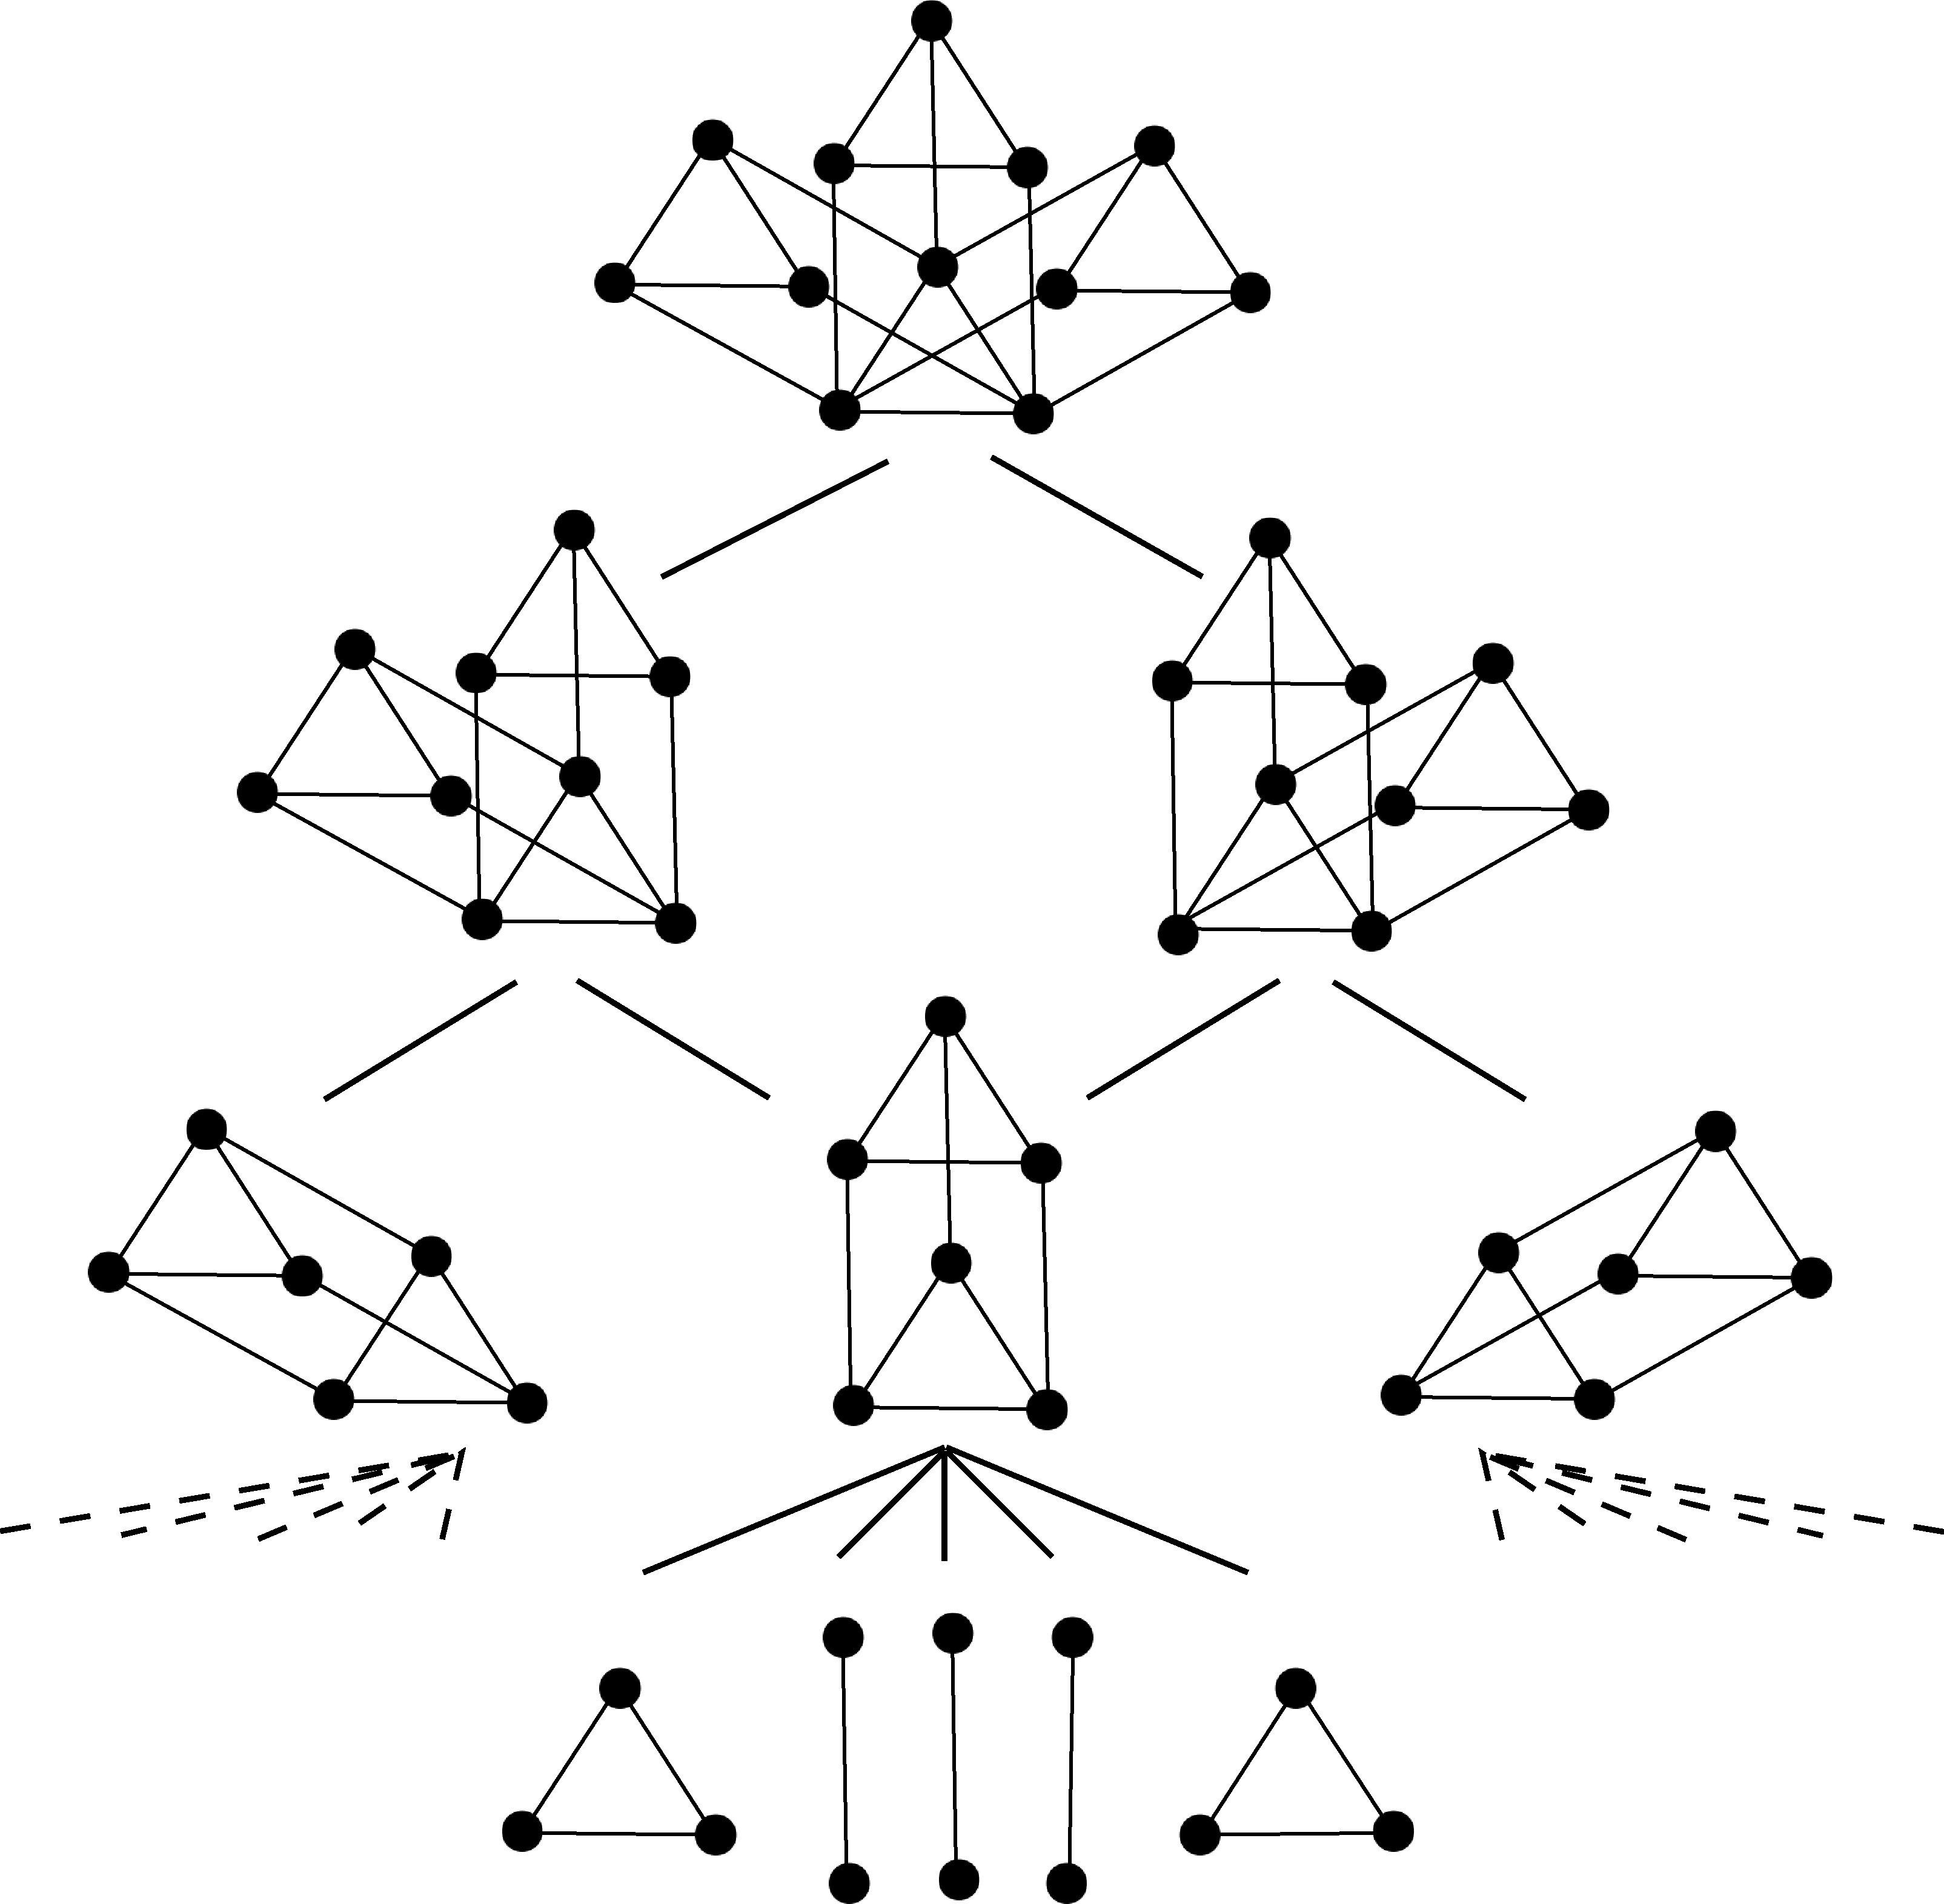
\includegraphics[width=.475\linewidth]{../../img/svg/3xc2c3_candrp_full} & 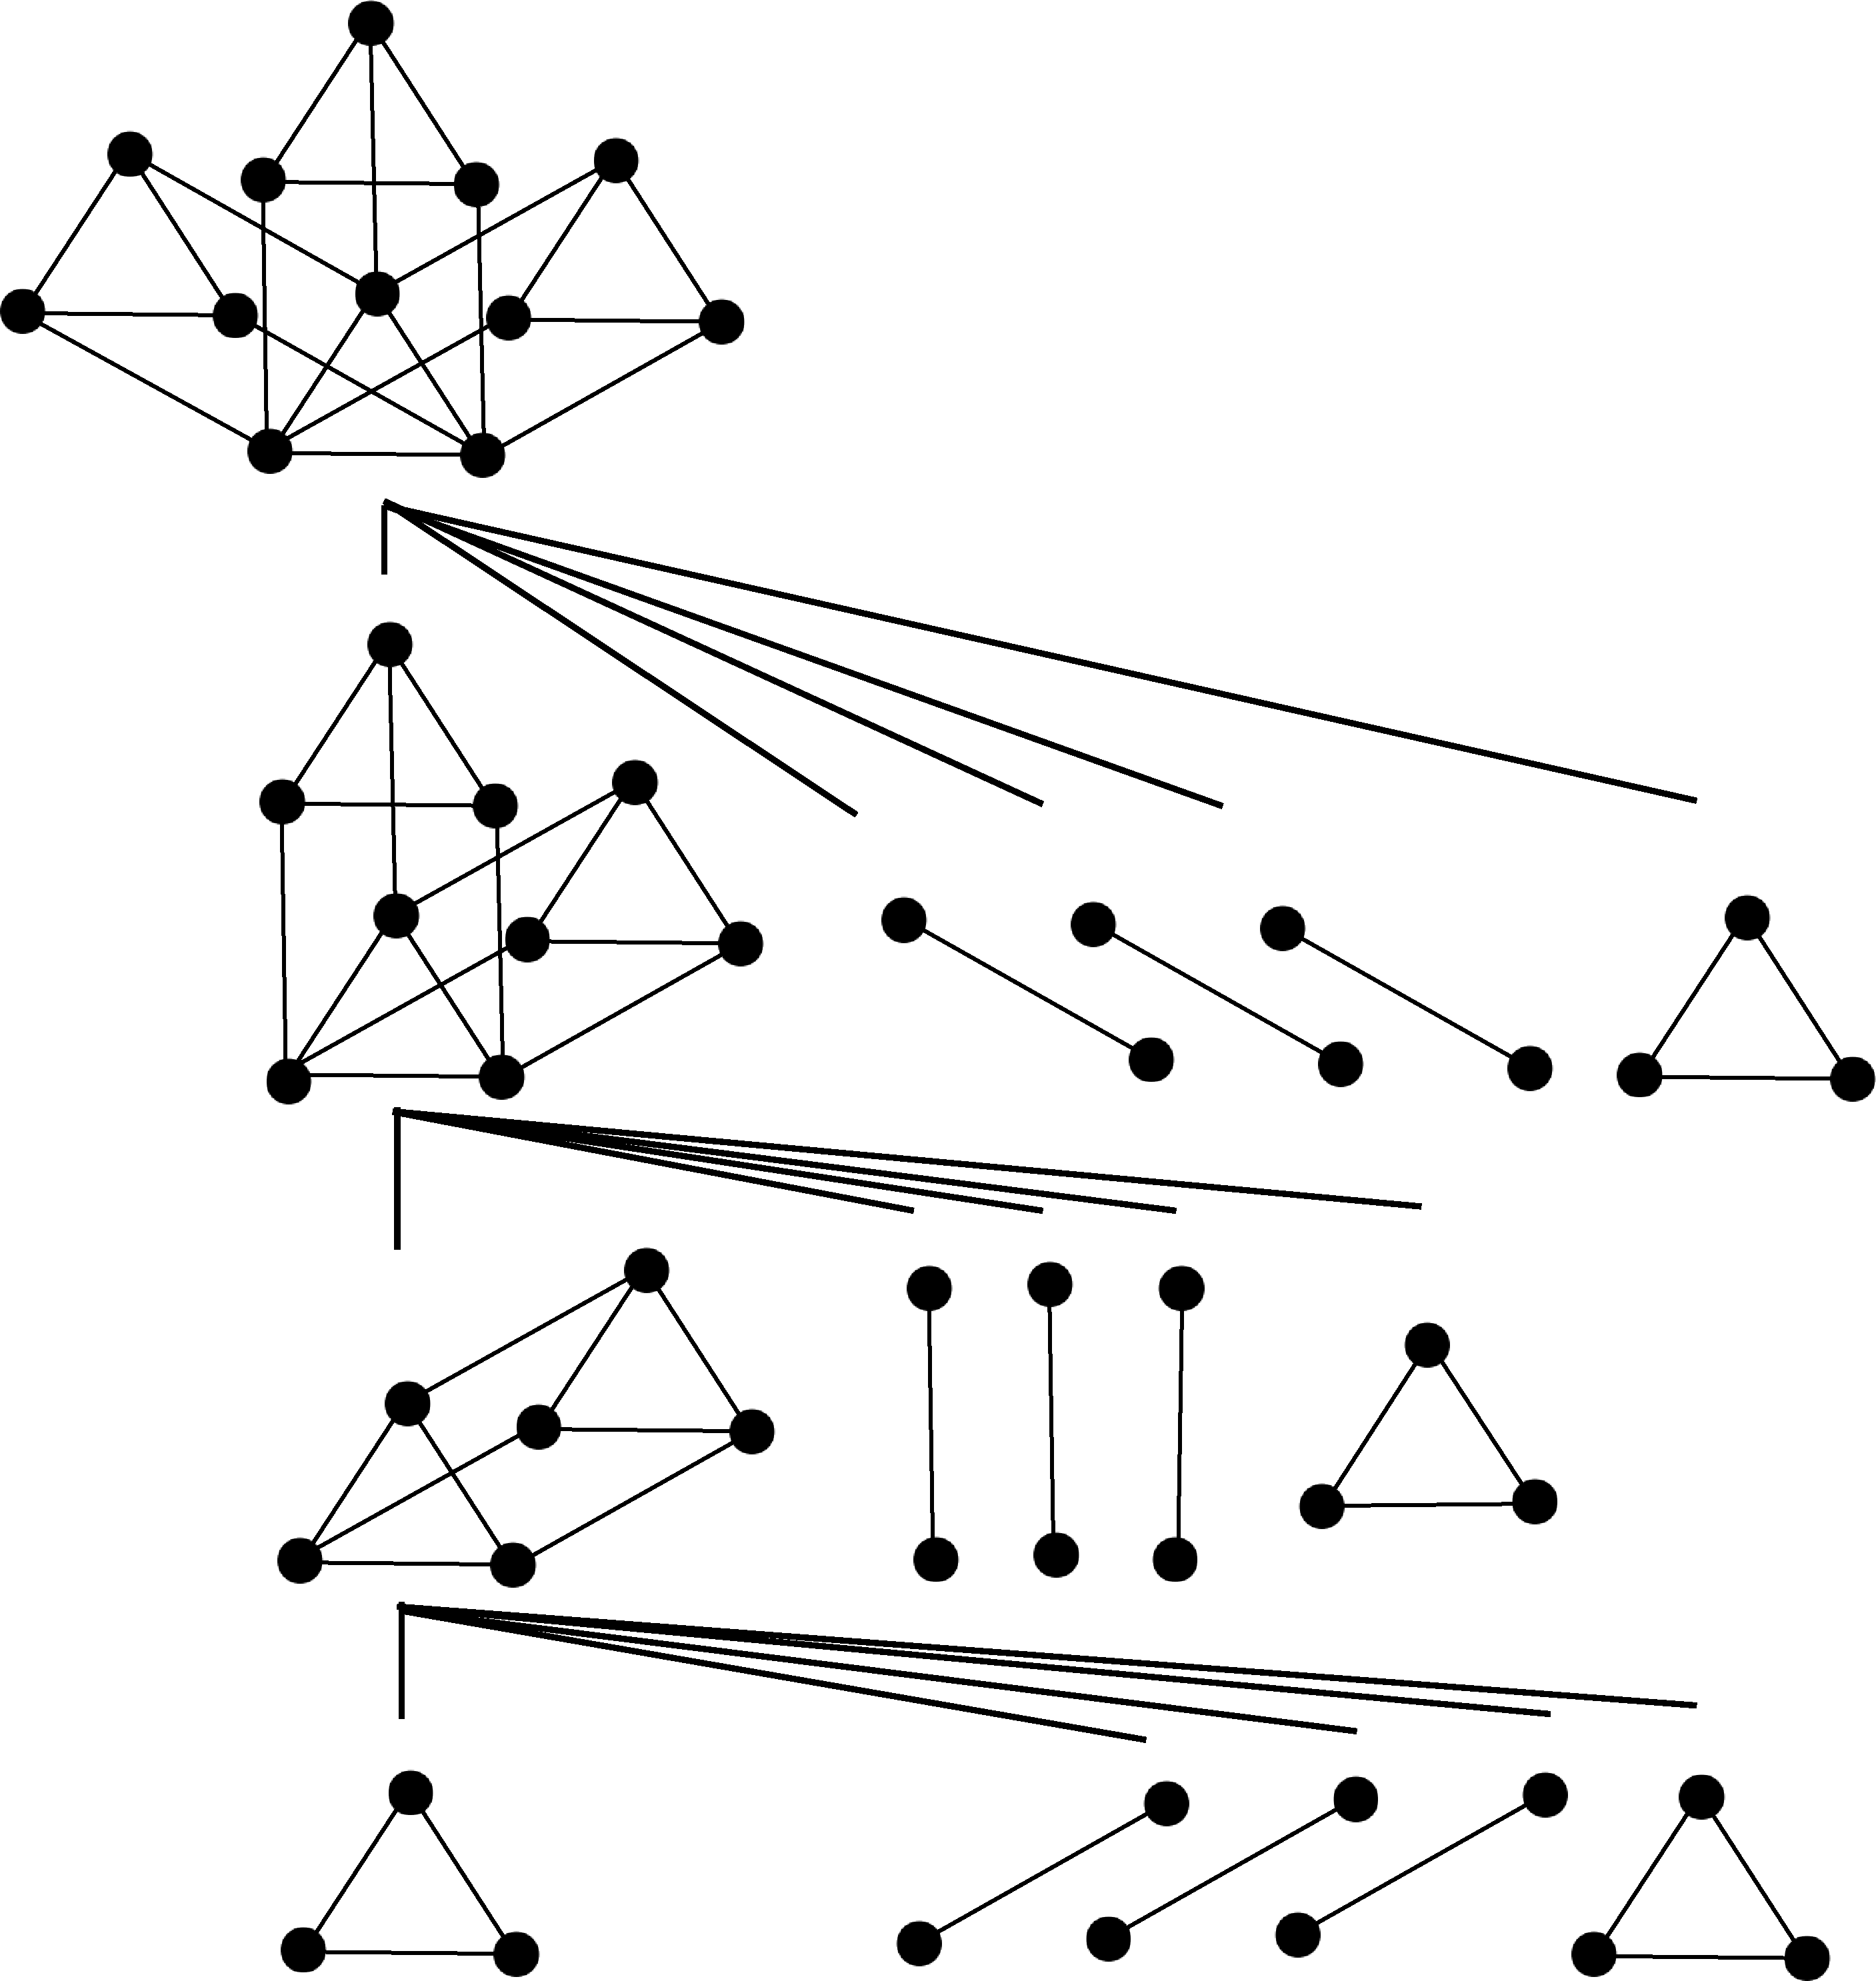
\includegraphics[width=.475\linewidth]{../../img/svg/3xc2c3_seqdrp_full}
    \end{tabular}
\end{frame}

\begin{frame}{Branches}
    \begin{definition}[Branch]
        Branch$(T,a,b)$ of tree $T$ is every node on the path from $a$ to $b$ and their children.
    \end{definition}

    % The leaves of the branch is exactly$^*$ the set of \rvmps\ of $a\setminus b$.

    % \n

    % The \rvmps\ can be found in time $O(|V|^2)$.

    \begin{figure}\centering
        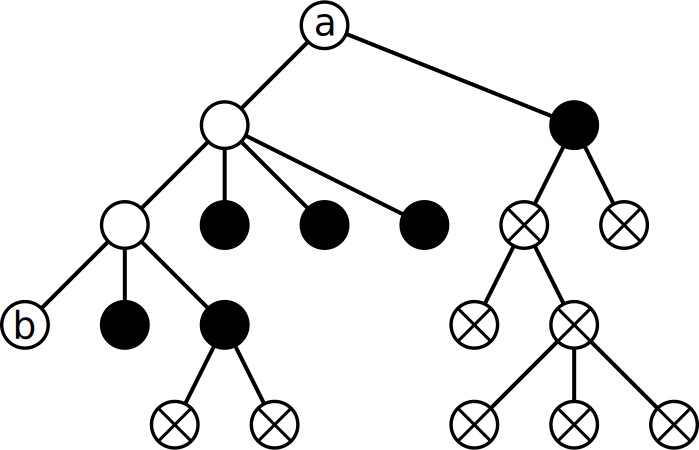
\includegraphics[width=.475\linewidth]{../../img/svg/branch_illustration}
    \end{figure}
\end{frame}

\begin{frame}{A Pseudosequential DR-Plan Branch from the Leaves}
    Given $G$ and $e\in G$, there exists a pseudosequential DR-plan $P_G$ where the leaves of branch$(P_G,G,e)$ is exactly$^*$ the \rvmps\ of $G\setminus e$.

    \pause
    \n

    We can find the \rvmps\ of $G\setminus e$ in $O(|V|^2)$.

    \pause
    \n

    Given a preprocessing step of finding the \rvmps\ of $G\setminus f$ for all $f$, branch$(P_G,G,e)$ can be built in time $O(|V|^2)$.

    \pause
    \n

    Building the branch (from $G$ to $e$):
    \begin{enumerate}
        \item Compute the \rvmps\ of $G\setminus e$, $\{L_i\}$.
        \item For each $L\in \{L_i\}$
        \begin{enumerate}
            \item Choose an arbitrary edge $f\in L$ and compute the \rvmps\ of $G\setminus f$, $\{M_i\}$.
            \item Compare the intersection of $L$ with each $M$ to get its position relative to the other leaves.
        \end{enumerate}
        \item Compute nodes on the path from $G$ to $e$.
    \end{enumerate}
\end{frame}

\begin{frame}{Finding an Entire Pseudosequential DR-Plan}
    Building the DR-plan (of $G$):
    \begin{enumerate}
        \item Preprocessing: Compute the \rvmps\ of $G\setminus e$, for all $e$.
        \item Start with $G$ as the single node in the DR-plan.
        \item Recursively compute a branch for each leaf in the DR-plan.
    \end{enumerate}
\end{frame}

% \begin{frame}{The Algorithm}
%     We can find the pseudosequential DR-plan by computing the \rvmps\ of $G\setminus e$, for all $e$ and doing a quadratic amount of work for each leaf.

%     \n

%     More specifically we:
%     \begin{enumerate}
%         \item Basis step: Start with $G$ as the single node in the DR-plan.
%         \item Recursive step: Compute a branch for each leaf in the DR-plan (that isn't a single edge.)
%         \begin{enumerate}
%             \item Choose arbitrary leaf $L$ and edge $f\in L$.
%             \item Compute the \rvmps\ of $L\setminus f$.
%             \item For each \rvmps, choose an arbitrary edge $g$ and compute the \rvmps\ of $L\setminus g$.
%             \item Compute the branch from $L$ to $f$ (uses a linear number of graph intersections to position each leaf.)
%         \end{enumerate}
%         % \begin{enumerate}
%         %     \item For each leaf $L$ and some edge $f\in L$, compute \rvmps\ of $G\setminus f$.
%         %      % (\rvmps\ of $L\setminus f$ are a subset.)
%         %     \item Compute the branch from $L$ to $f$ (uses a linear number of graph intersections.)
%         % \end{enumerate}
%     \end{enumerate}
% \end{frame}

\begin{frame}{Algorithm Demonstration}
    \begin{figure}
        \includegraphics<1>[width=0.08\linewidth]{../../img/svg/algo_illustration_a}
        \includegraphics<2>[width=0.75\linewidth]{../../img/svg/algo_illustration_b}
        \includegraphics<3>[width=0.75\linewidth]{../../img/svg/algo_illustration_c}
        \includegraphics<4>[width=0.75\linewidth]{../../img/svg/algo_illustration_d}
        \includegraphics<5>[width=0.75\linewidth]{../../img/svg/algo_illustration_e}
        \includegraphics<6>[width=0.75\linewidth]{../../img/svg/algo_illustration_f}
    \end{figure}
\end{frame}

\begin{frame}{Finding an Entire Pseudosequential DR-Plan}
    Building the DR-plan (of $G$):
    \begin{enumerate}
        \item Preprocessing: Compute the \rvmps\ of $G\setminus e$, for all $e$.
        \item Start with $G$ as the single node in the DR-plan.
        \item Recursively compute a branch for each leaf in the DR-plan.
    \end{enumerate}
\end{frame}

\begin{frame}{Open Source Software}
    Under development.
    % \footfullcite{baker2015arxiv}

    Current version available at: \url{cise.ufl.edu/~tbaker/drp}
    \begin{figure}\centering
        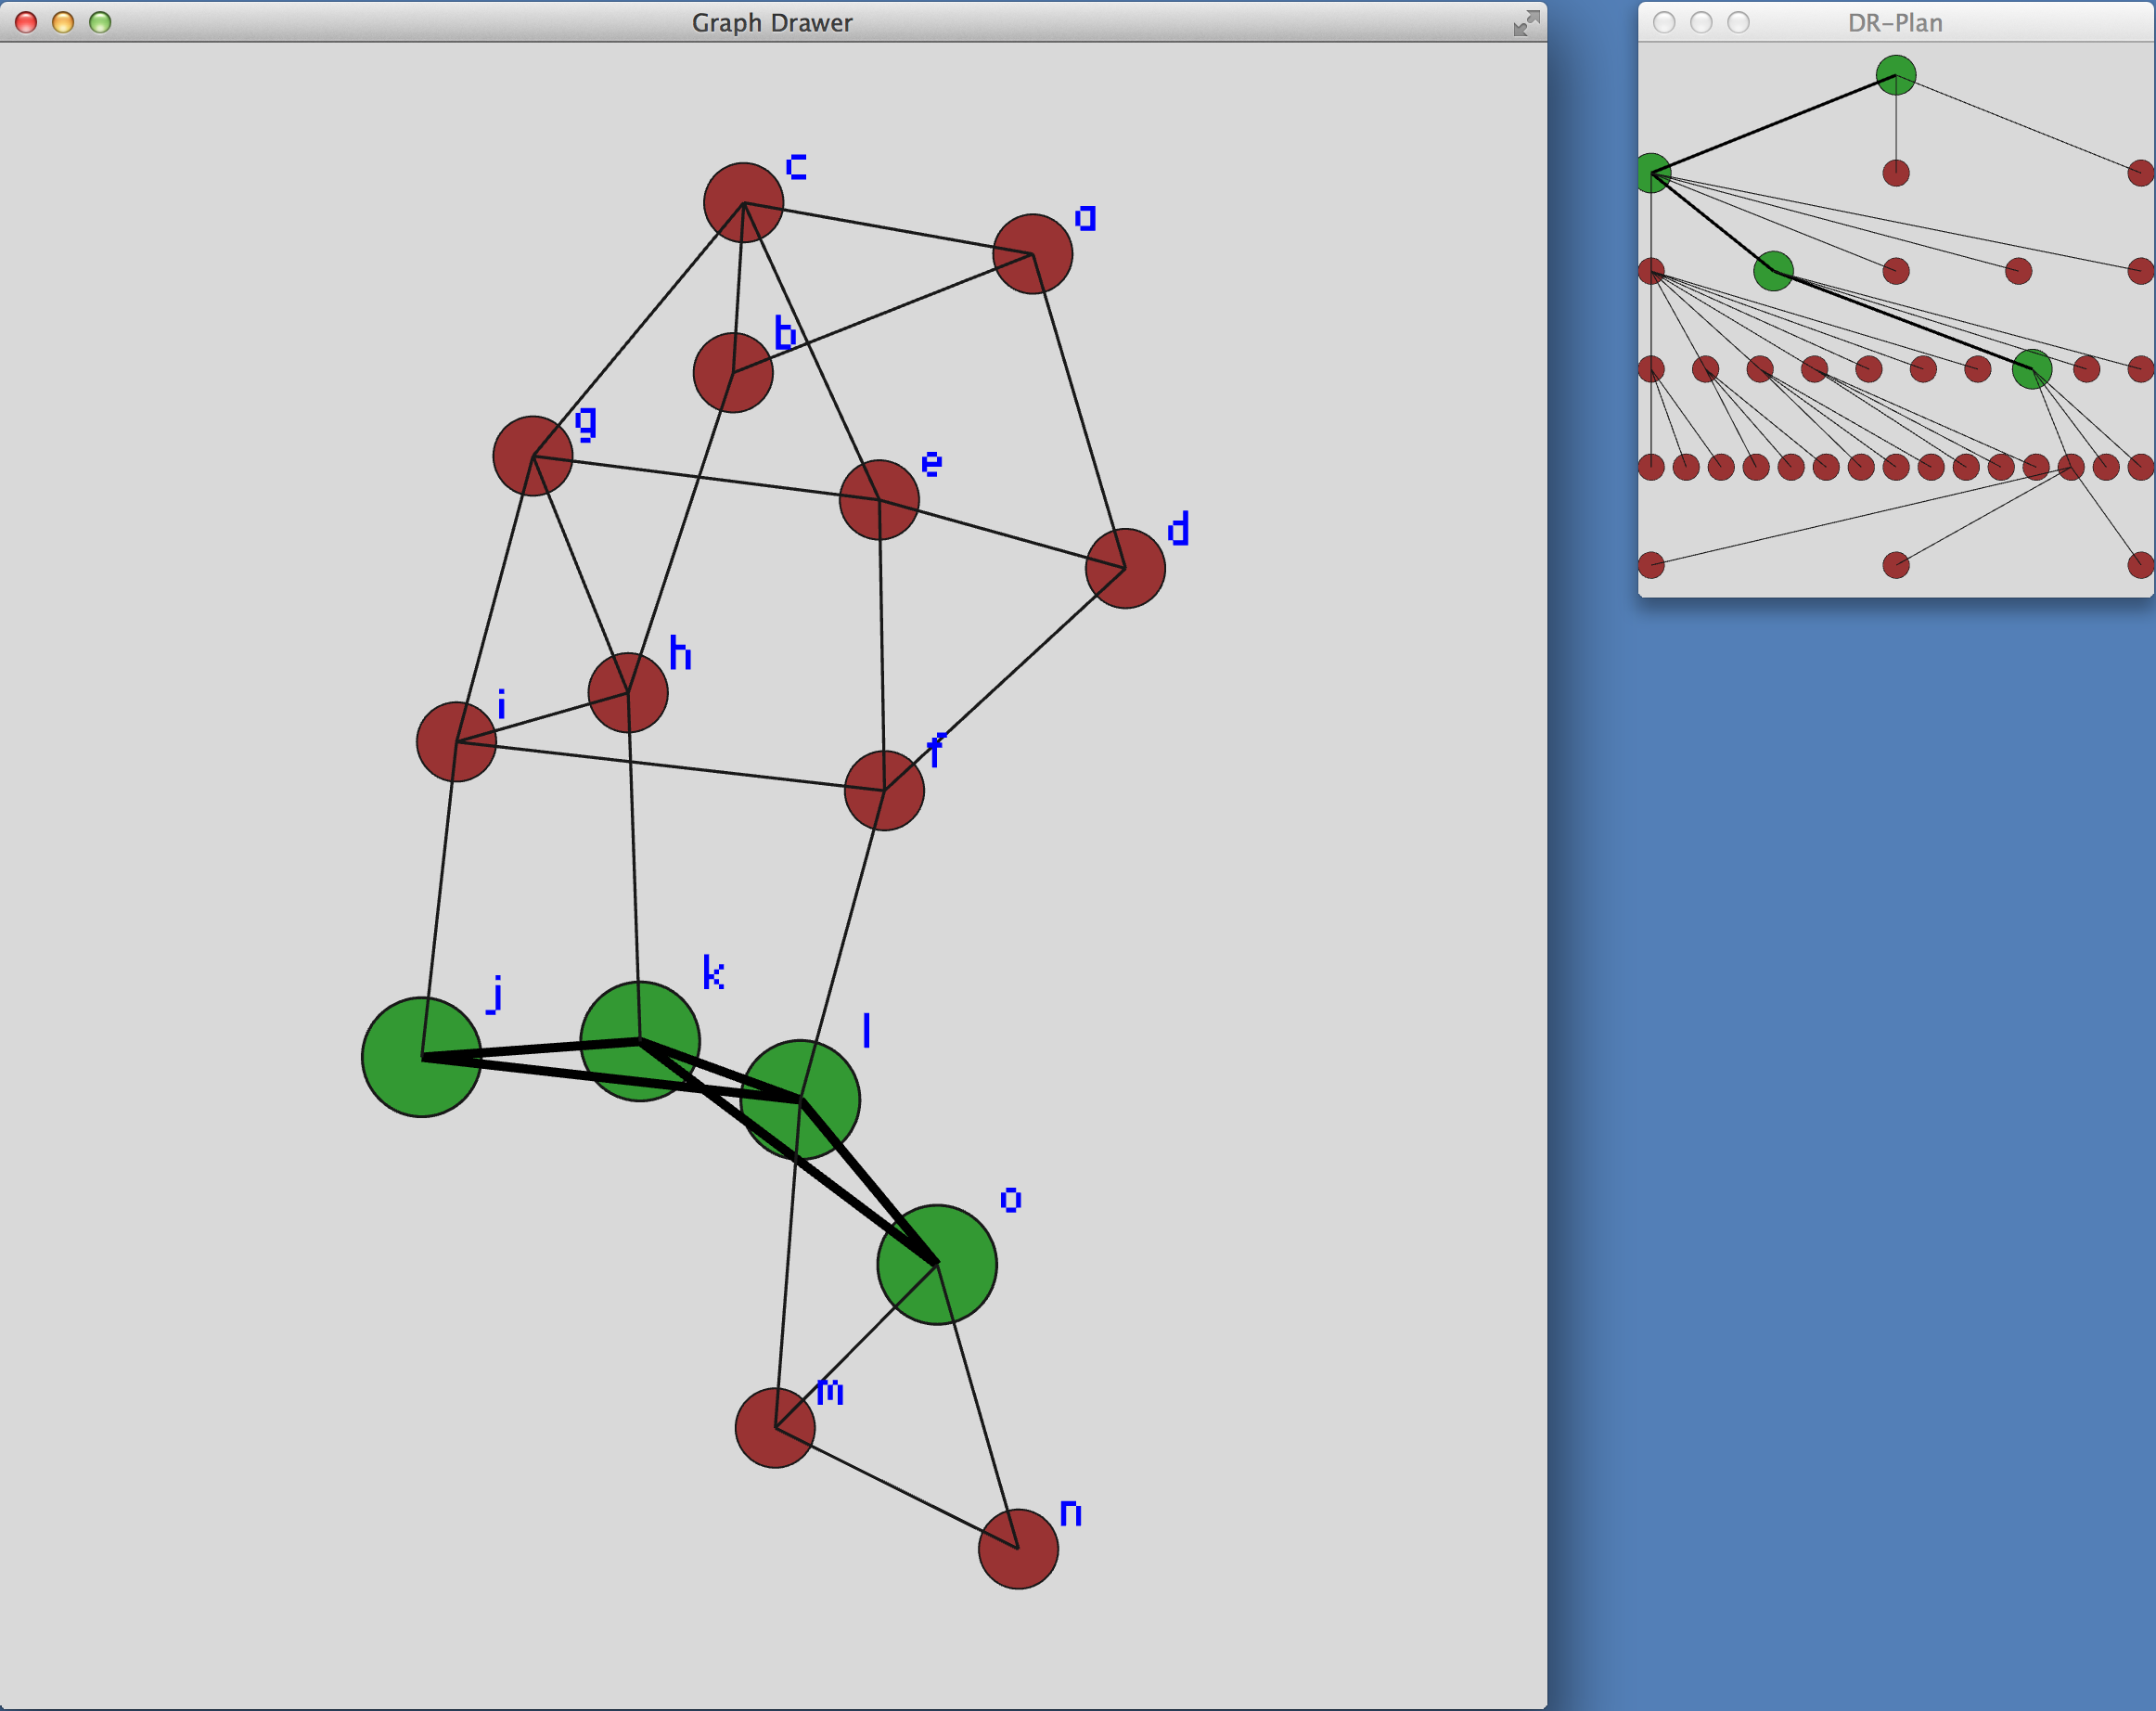
\includegraphics[width=0.65\linewidth]{../../img/screenshots/node_in_drp}
    \end{figure}
\end{frame}

\section{Main Result: OMD}
\begin{frame}{What Next?}
    What comes after optimal DR-planning? We've decomposed to the extent possible.

    \n

    Na{\"i}vely, we would, bottom-up, recombine the solved children into parents.

    % \n

    % Recombining each node is equivalent to solving an indecomposable system.


    % Subsystems of any given node have solutions. We are trying to recombine these solved subsystems to get the parent.

    % \n

    % This is equivalent to solving an indecomposable system. Na{\"i}vely we would just start solving.
\end{frame}

\begin{frame}{OMD}
\small
    \begin{definition}[Optimal modification for decomposition (OMD)]
        % OMD$(G,k,s)$ asks if there exist $k$ edges to drop from $G$ and some set of edges to add to $G$, such that the new graph has a DR-plan of max fan-in $s$.
        Informally, can we drop some edges and add some others to make an easily realizable system (i.e.\ small max fan-in DR-plan)?
    \end{definition}

    % Added edges parameterize the realization space, which we search for a realization that satisfies the dropped constraints.

    % \n

    Dropped edges: Chosen so that the realization space has a convex parameterization.
    % \todo{citation}
    % We know how to find dropped edges so that the realization space has a convex parameterization, which can be efficiently searched.

    \n

    Added edges: Parameterize the realization space. Chosen so that the realization can be efficiently computed (e.g., triangle-decomposable.)

    \n

    We search the realization space for those that satisfy the dropped constraints.

    % We can efficiently compute the realization because of the edges we chose to add.


    \begin{figure}
        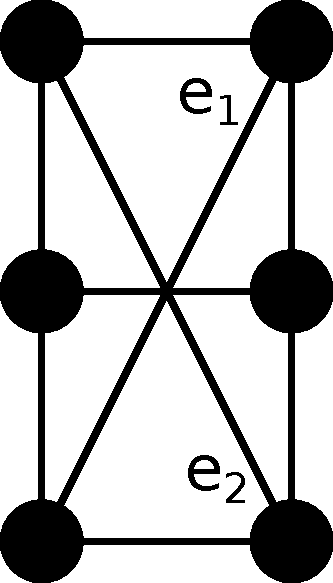
\includegraphics[height=0.23\linewidth]{../../img/svg/k33_omd_a}
        \hspace{3em}
        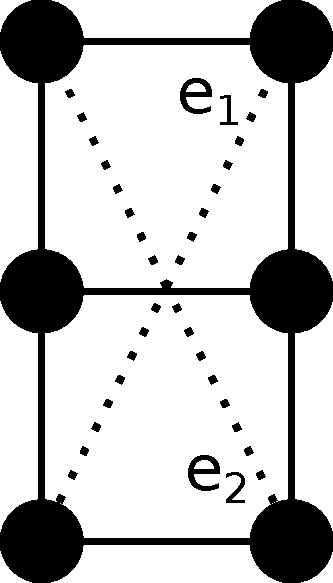
\includegraphics[height=0.23\linewidth]{../../img/svg/k33_omd_b}
        \hspace{3em}
        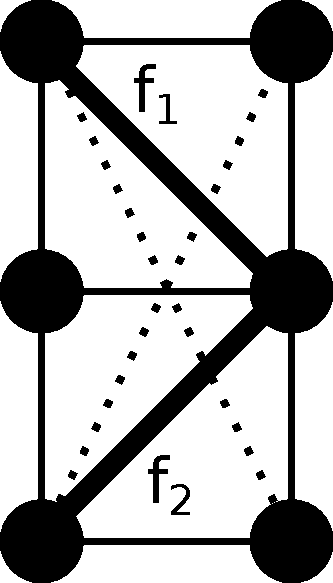
\includegraphics[height=0.23\linewidth]{../../img/svg/k33_omd_c}
    \end{figure}
\end{frame}

\begin{frame}{Open Problems}
    \begin{openproblem}
        Is there a more efficient algorithm than $O(|V|^3)$ to find the canonical DR-plan of isostatic 2D bar-joint graphs?
    \end{openproblem}

    \begin{conjecture}
    \label{conj:mfaisoptimal:rephrase}
        For independent graphs, \term{cluster-minimal} DR-plans are optimal. In fact, for independent graphs, cluster-minimality and canonical are equivalent properties of a DR-plan.
    \end{conjecture}

    Additional problems can be found in the paper.
\end{frame}


% --------------------------------------------------------------
%                        End of Body
% --------------------------------------------------------------


\begin{frame}[allowframebreaks]{Bibliography}
    \bibliographystyle{plain}
    \bibliography{references}
    % \printbibliography
\end{frame}

% \bibliographystyle{plain}
% \bibliography{references}

\end{document}

% --------------------------------------------------------------
%                       End of Document
% --------------------------------------------------------------
